\chapter{Results:}

Tables \ref{amplSum26} and \ref{amplSum70} summarise the seasonal amplitude of all defined variables averaged over the last simulation decade, without and with alkalinity enhancement, for the European coastline and for location S under both emission scenarios. Below, each variable is then investigated in depth. 

\begin{center}

\begin{table}[H]
\captionof{table}[Seasonal amplitude average for alkalinity, pH, \texorpdfstring{DIC}{DIC}, \ch{pCO2}, and \ch{CO2} flux in SSP1-2.6.]{For SSP1-2.6, seasonal amplitude for alkalinity, pH, \ac{dic}, \ch{pCO2}, and \ch{CO2} flux averaged over 2090 to 2100.
\label{amplSum26}}

\scalebox{0.95}{
        \begin{tabular}{|| c || c c || c c || c ||} % c|l|r
    {} & \multicolumn{2}{c}{European average} 
    & 
    \multicolumn{2}{c}{Location S} \\
    {} & {Without \ac{oae}} & {With \ac{oae}} & {Without \ac{oae}} & {With \ac{oae}} & {Unit} \\
    \hline \hline
    {} & {} & {} & {} & {} \\
    Alkalinity & 11 & 5 & 25 & 215 & mmol m\textsuperscript{-3} \\
    pH & 0.027 & 0.017 & 0.139 & 0.143 & - \\
    \ac{dic} & 30 & 23 & 46 & 54 & mmol m\textsuperscript{-3} \\
    \ch{pCO2} & 35 & 23 & 166 & 51 & µatm \\
    \ch{CO2} flux & 2.69 & 3.88 & 8.17 & 16.49 & mol m\textsuperscript{-2} yr\textsuperscript{-1} \\
    \end{tabular}}
\end{table}

\end{center}

\begin{center}

\begin{table}[H]
\captionof{table}[Seasonal amplitude average for alkalinity, pH, \texorpdfstring{DIC}{DIC}, \ch{pCO2}, and \ch{CO2} flux in SSP3-7.0.]{For SSP3-7.0, seasonal amplitude for alkalinity, pH, \ac{dic}, \ch{pCO2}, and \ch{CO2} flux averaged over 2090 to 2100.\label{amplSum70}}

\scalebox{0.95}{
        \begin{tabular}{|| c || c c || c c || c ||} % c|l|r
    {} & \multicolumn{2}{c}{European average} 
    & 
    \multicolumn{2}{c}{Location S} \\
    {} & {Without \ac{oae}} & {With \ac{oae}} & {Without \ac{oae}} & {With \ac{oae}} & {Unit} \\
    \hline \hline
    {} & {} & {} & {} & {} \\
    Alkalinity & 13 & 6 & 44 & 354 & mmol m\textsuperscript{-3} \\
    pH & 0.029 & 0.018 & 0.099 & 0.159 & - \\
    \ac{dic} & 27 & 17 & 74 & 136 & mmol m\textsuperscript{-3} \\
    \ch{pCO2} & 73 & 55 & 207 & 112 & µatm \\
    \ch{CO2} flux & 4.34 & 6.38 & 9.24 & 28.26 & mol m\textsuperscript{-2} yr\textsuperscript{-1} \\
        \end{tabular}}
\end{table}

\end{center}

\section{Alkalinity:}

\begin{figure}[H]
\caption[Monthly average of baseline and \texorpdfstring{OAE}{OAE}-induced alkalinity]{From left to right, monthly average of baseline and \ac{oae}-induced alkalinity (mmol m\textsuperscript{-3}) in the European region in SSP1-2.6 (A), and in SSP3-7.0 (C), and at location S in SSP1-2.6 (E) and in SSP3-7.0 (G) averaged over 2090-2100 (top), and the difference ($\Delta$) (B, D, F, and H) between the two scenarios (bottom).}
\label{alkalinity}
\centering
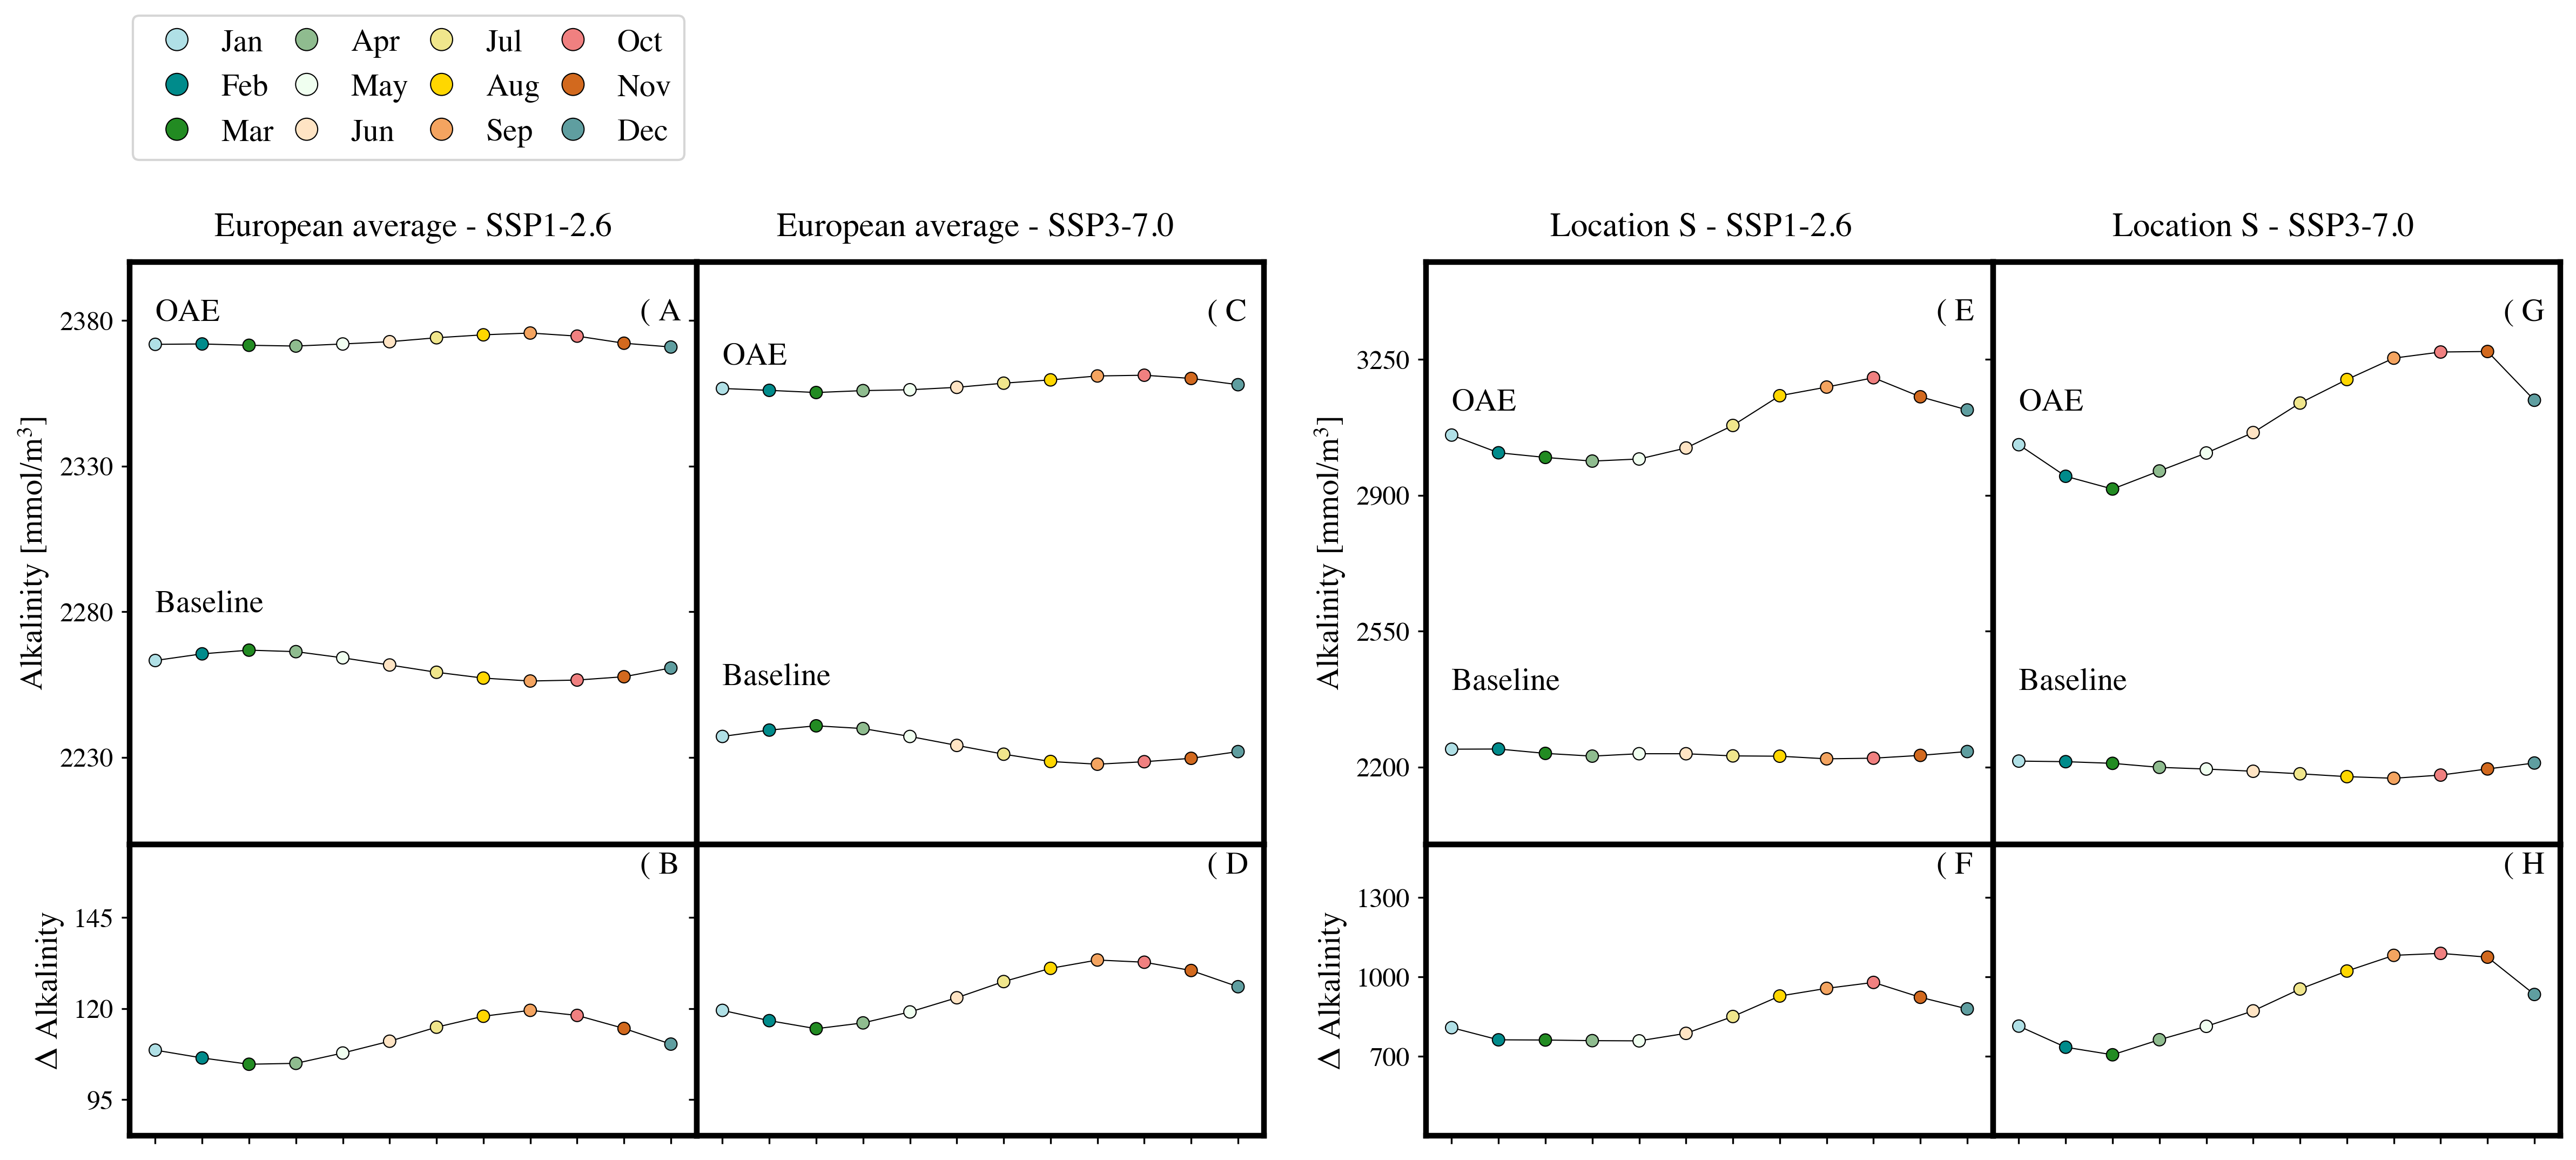
\includegraphics[width=15cm]{fig/3_Results/Alkalinity/alkalinity.png}

\end{figure}

The baseline alkalinity seasonality in SSP1-2.6 in the European region stretches between highest values at the onset of spring and lowest values in autumn. Maxima and minima are recorded in March and October, respectively. The average amplitude spans between 2256 and 2267 mmol m\textsuperscript{-3}. In the \ac{oae} scenario, absolute values of alkalinity ramp up due to alkalinity addition. A of \cref{alkalinity} portrays a flattening of the line and seasonality is halved, with a current mean amplitude of 5 mmol m\textsuperscript{-3}. Lowest and highest alkalinity are now recorded in April and September, respectively (C of \cref{alkalinity}), revealing a strong alteration of the baseline seasonal cycle. The baseline high-emission scenario displays absolute values that are slightly lower than SSP1-2.6, with a mean seasonal range between 2228 and 2241 mmol m\textsuperscript{-3} in summer and winter, respectively. Similar to SSP1-2.6, alkalinity enhancement forces the annual cycle to a shift, where maxima are displayed in November and minima in March, with a decreased amplitude of 6 mmol m\textsuperscript{-3}. 

At location S in SSP1-2.6, \ac{oae} induces alkalinity absolute values to rise greatly and, unlike the European mean, the annual amplitude is enhanced (E of \cref{alkalinity}). The annual cycle shifts to high peaks in October and bottom peaks in April with an average range between 2988 and 3203 mmol m\textsuperscript{-3}, therefore exceeding by far the baseline amplitude of only 25 mmol m\textsuperscript{-3}. Higher atmospheric \ch{CO2} concentrations magnify the observed seasonal amplification (G of \cref{alkalinity}). Additionally, all $\Delta$ (B, D, F, and H of \cref{alkalinity}) reveal the highest baseline-to-\ac{oae} variation between September and October.

\begin{figure}[H]
\caption[European monthly average of baseline and \texorpdfstring{OAE}{OAE}-induced alkalinity as a function of depth]{European monthly average of baseline and \ac{oae}-induced alkalinity (mmol m\textsuperscript{-3}) as a function of depth (m) averaged over 2090-2100 (left). Grey lines define the \ac{foci} ocean layers. European monthly average of alkalinity (mmol m\textsuperscript{-3}) at the first \ac{foci} layer over 2090-2100 (right).}
\label{EUalkalinitysurface}
\centering
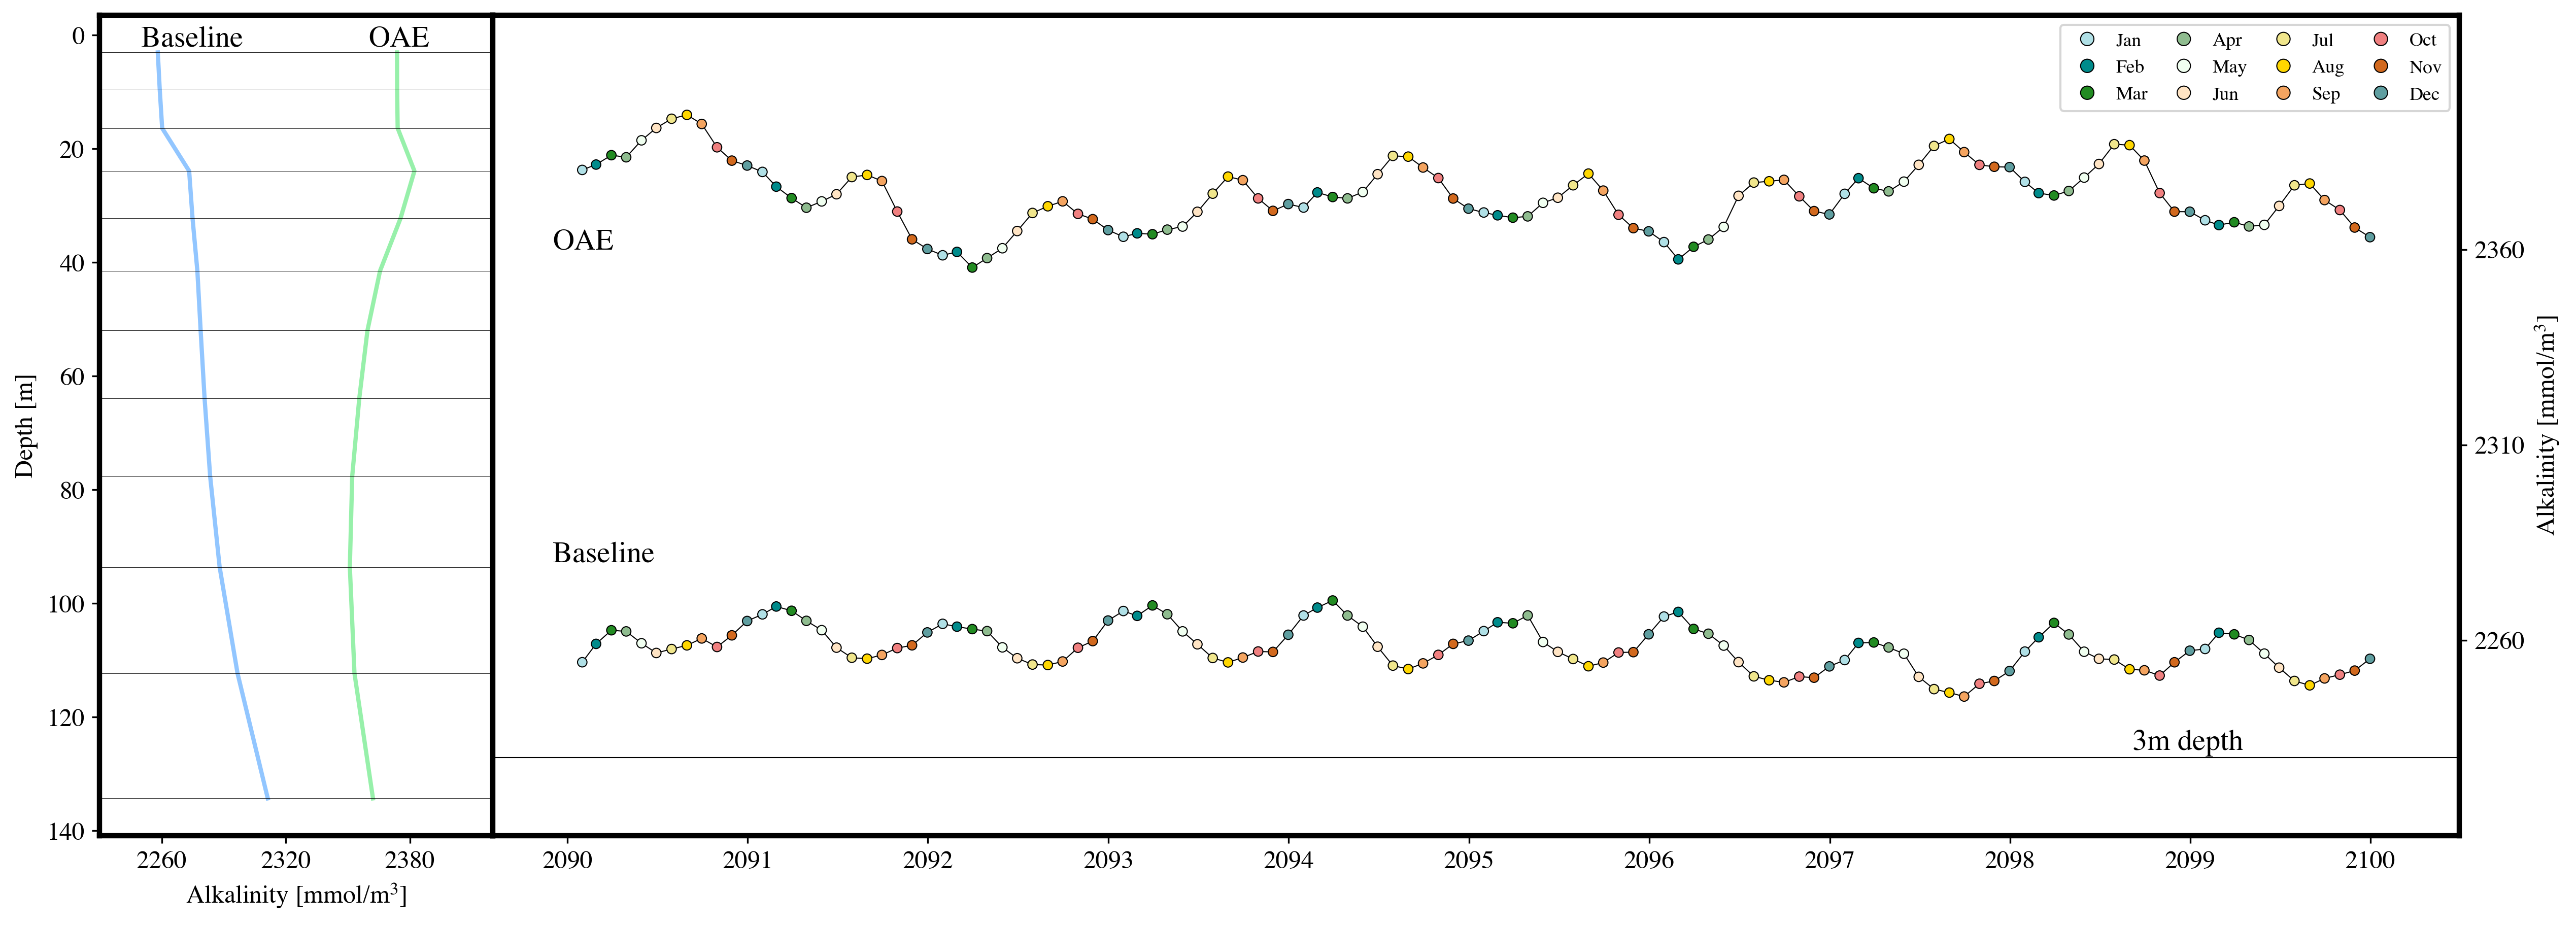
\includegraphics[width=15cm]{fig/3_Results/Alkalinity/EUAlk_depthprof.png}

\end{figure}

To explain the seasonal cycle alteration visible in A and C of \cref{alkalinity}, \cref{EUalkalinitysurface} shows the decadal mean of alkalinity for the first 3 metres of the ocean surface, where an evident reversal is recorded (right). On the left graph, alkalinity is plotted as a function of depth: the baseline values increase when moving deeper whereas the \ac{oae} has highest alkalinity at the surface (where it is added in the experiments) and progressively decreases up to about 90 metres, when it starts rising again. The reason for such a diversion is connected with the alteration of the alkalinity natural distribution through water column. 

\begin{figure}[H]
\caption[Alkalinity seasonal amplitude change]{Alkalinity seasonal amplitude change (mmol m\textsuperscript{-3}) without \ac{oae} (left), with \ac{oae} (middle), and the difference ($\Delta$) between the two (right). SSP1-2.6 (top) and SSP3-7.0 (bottom).}
\label{alkalinityamplitude}
\centering
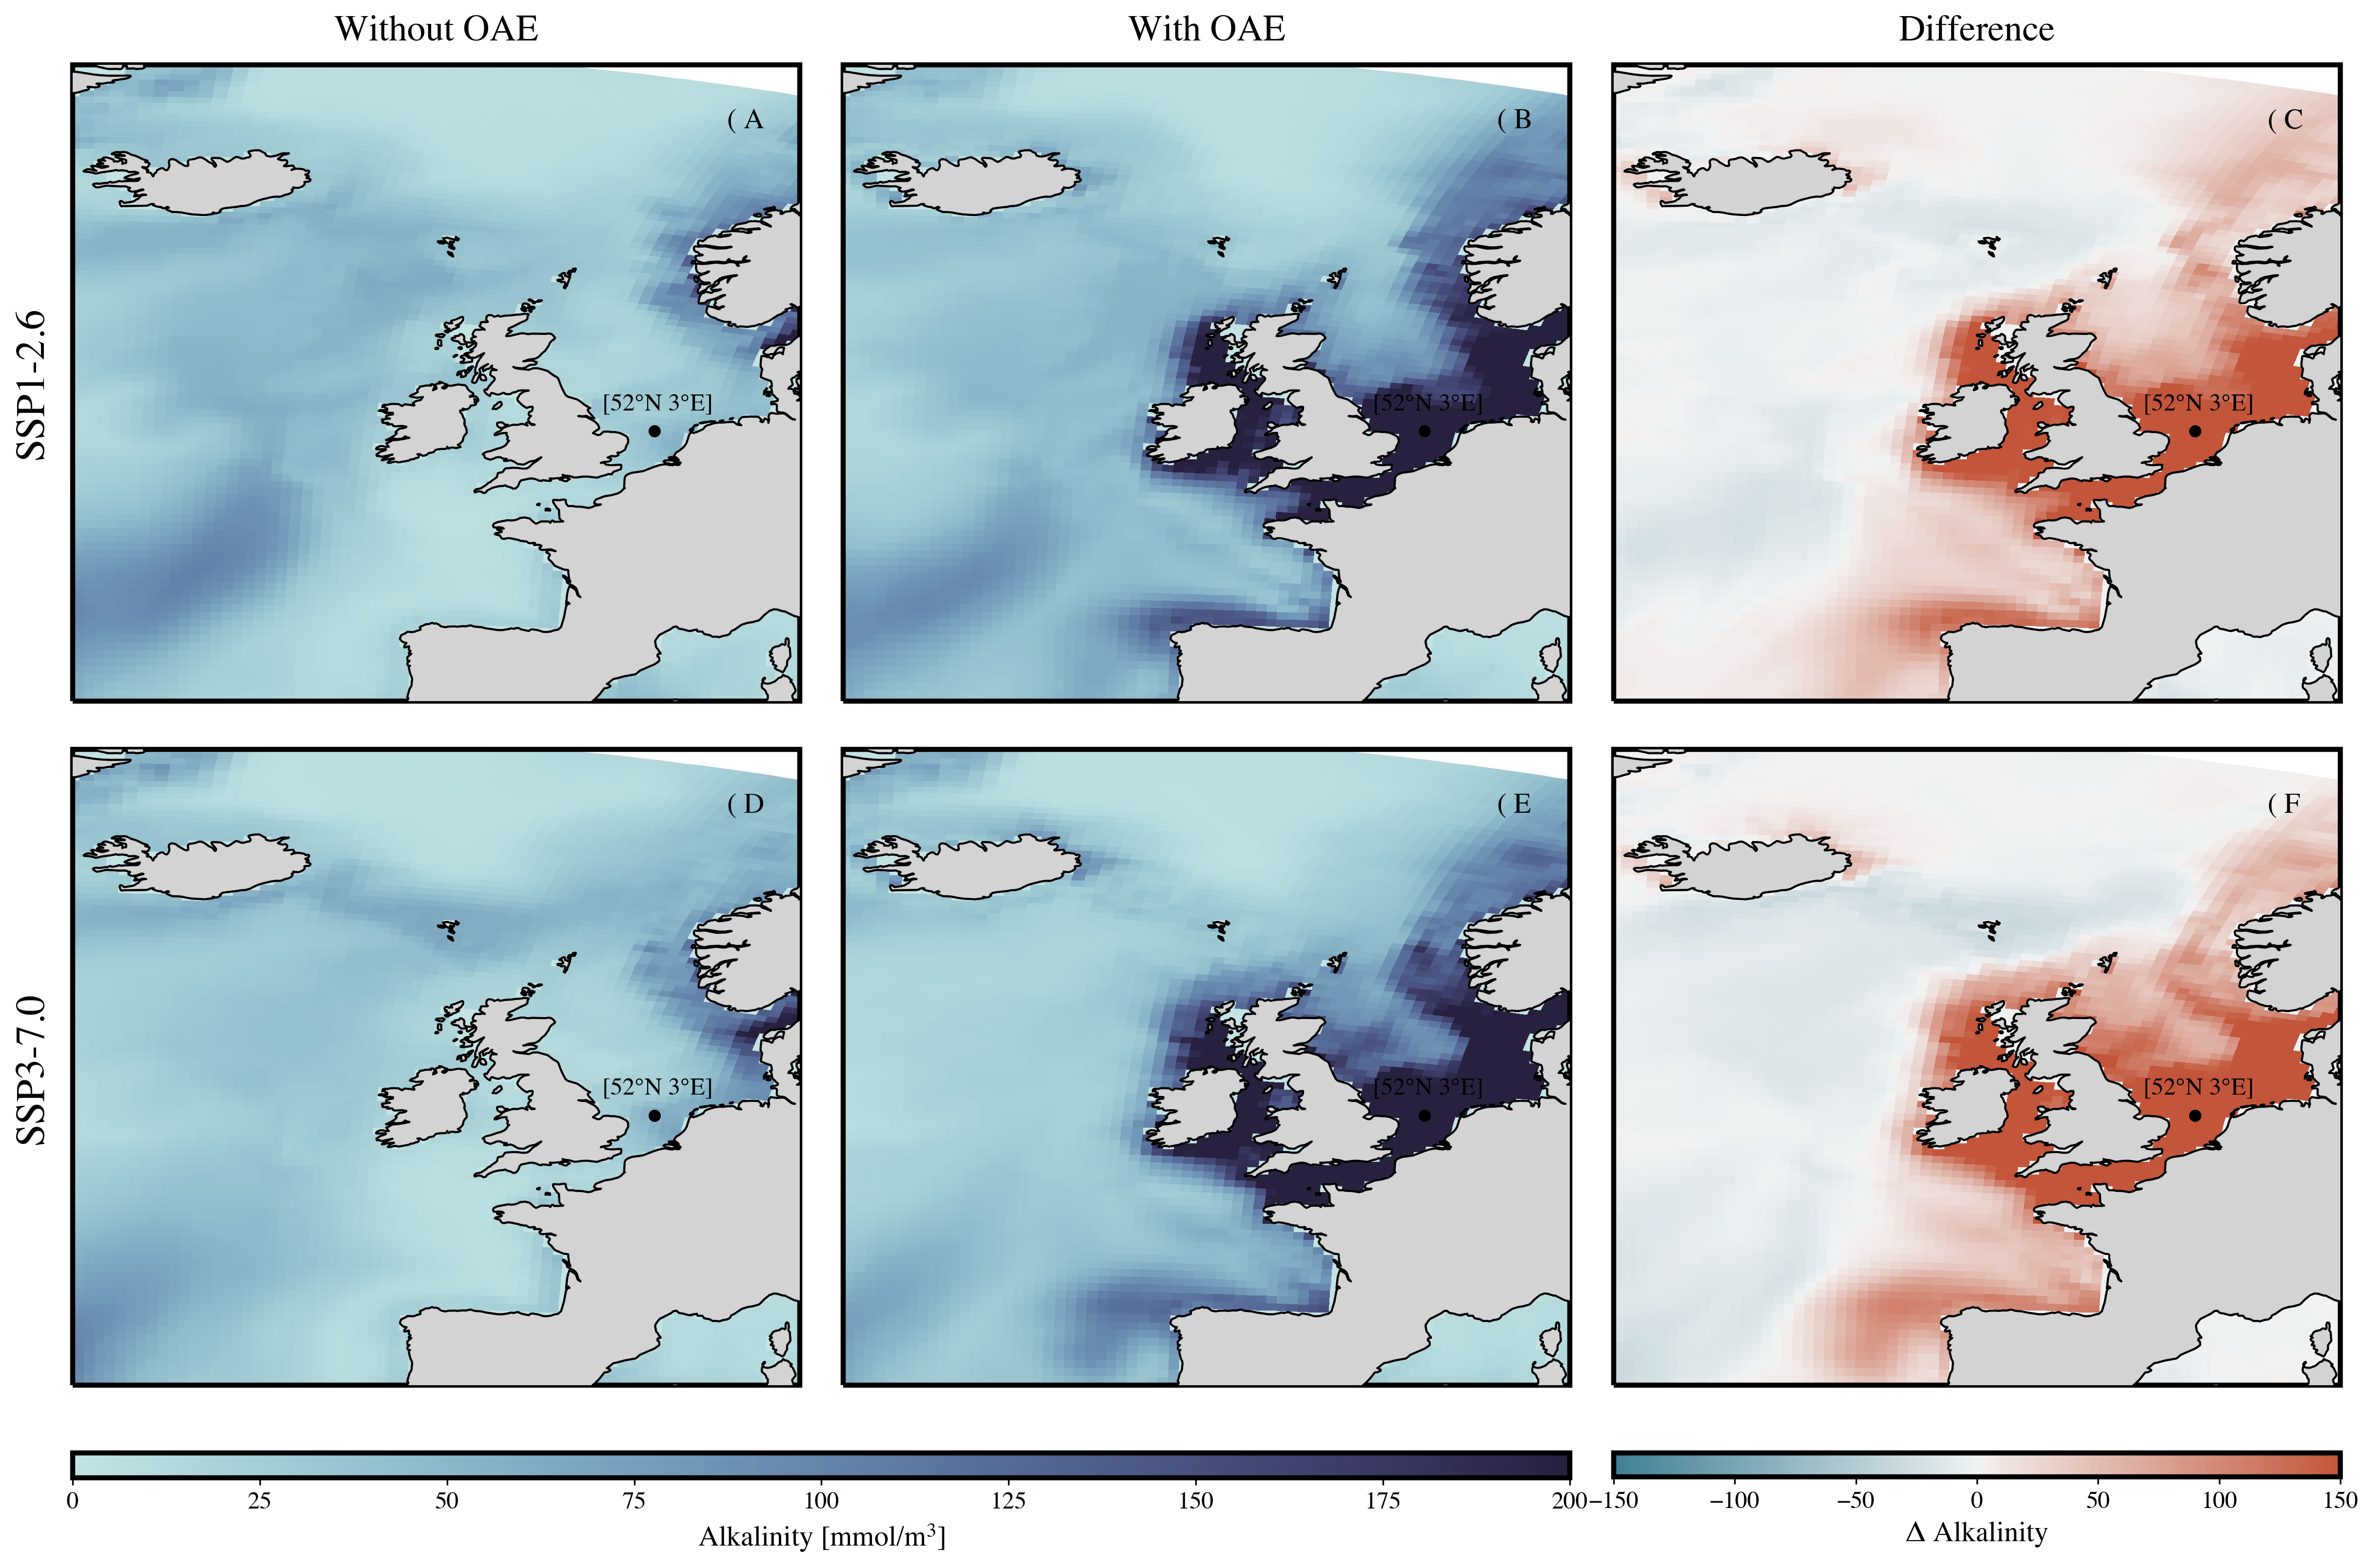
\includegraphics[width=15cm]{fig/3_Results/Alkalinity/alkalinity_ampl.png}

\end{figure}

In both scenarios, alkalinity addition operates to expand the seasonal amplitude only at the proximity of the injection site, especially at the UK littoral and in the southern and central North Sea (red regions in C and F of \cref{alkalinityamplitude}). The coasts of southern Norway and northern Spain represent an exception, where poor variation in amplitude is shown. Iceland reflects almost no change and its southern shoreline joins the pattern of the open ocean which displays a modest decreasing trend (light blue regions). In SSP3-7.0, the seasonal amplitude expands further than the low emission scenario, though maintaining the same pattern.

\section{pH:}

\begin{figure}[H]
\caption[Monthly average of baseline and \texorpdfstring{OAE}{OAE}-induced pH]{From left to right, monthly average of baseline and \ac{oae}-induced pH in the European region in SSP1-2.6 (A), and in SSP3-7.0 (C), and at location S in SSP1-2.6 (E) and in SSP3-7.0 (G) averaged over 2090-2100 (top), and the difference ($\Delta$) (B, D, F, and H) between the two scenarios (bottom).}
\label{ph}
\centering
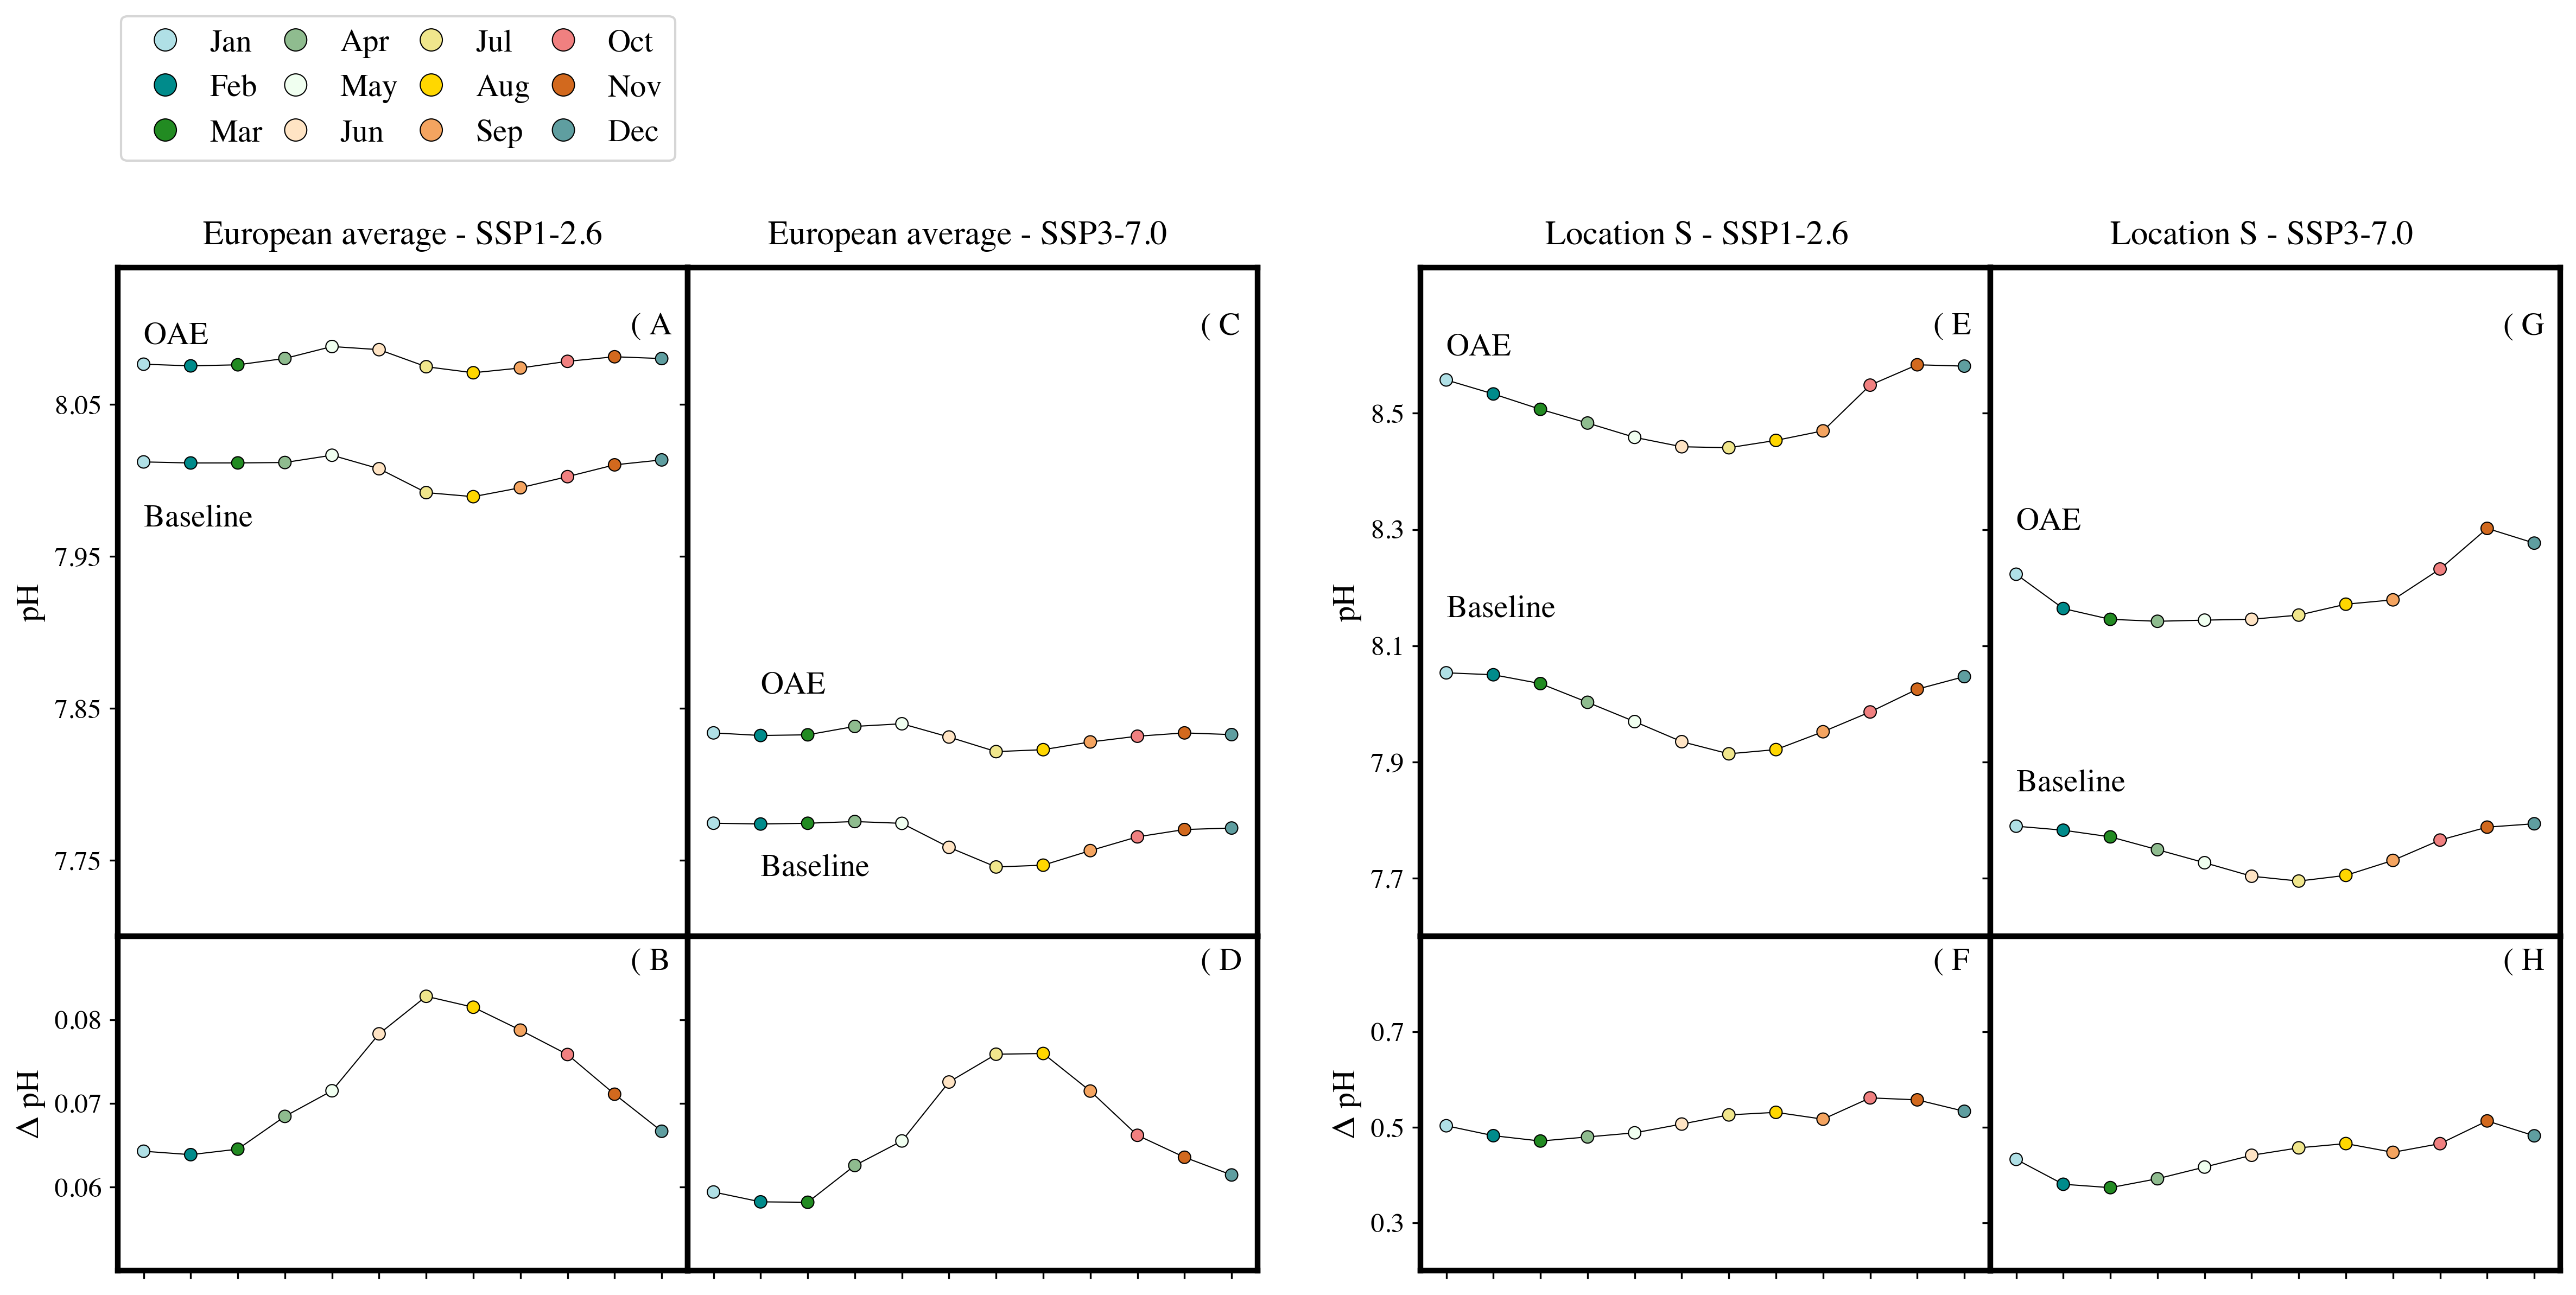
\includegraphics[width=15cm]{fig/3_Results/pH/ph.png}

\end{figure}

At the European average in SSP1-2.6, baseline pH reveals maxima in spring, reaching 8.01 units, and minima in summer, when it drops to 7.99. pH levels increase when \ac{oae} is employed and the amplitude is reduced by 0.01 units. This slight compression is due to \ac{oae} being most efficient at highest seawater acidification, that is, in summer months (B of \cref{ph}). In SSP3-7.0, pH absolute values are lower due to enhanced anthropogenic \ch{CO2} inputs to the atmosphere and a decreasing trend is registered until the end of the century (not shown). The seasonal amplitude change is maintained, with a minimal dampening compared to the baseline. 

At location S in SSP1-2.6, \ac{oae} is able to rise pH to values as high as over 8.5 units, with a nearly uniform increase throughout the year (F of \cref{ph}). In SSP3-7.0, \ac{oae} is able to restore pH levels, although not as efficiently as in the low-emission scenario. In both climate states, $\Delta$ pH reaches its peak in November, when highest alkalinity is detected (E and G of \cref{alkalinity}), showing a fast response to \ac{oae} perturbations. 

\begin{figure}[H]
\caption[pH seasonal amplitude change]{pH seasonal amplitude change without \ac{oae} (left), with \ac{oae} (middle), and the difference ($\Delta$) between the two (right). SSP1-2.6 (top) and SSP3-7.0 (bottom).}
\label{phamplitude}
\centering
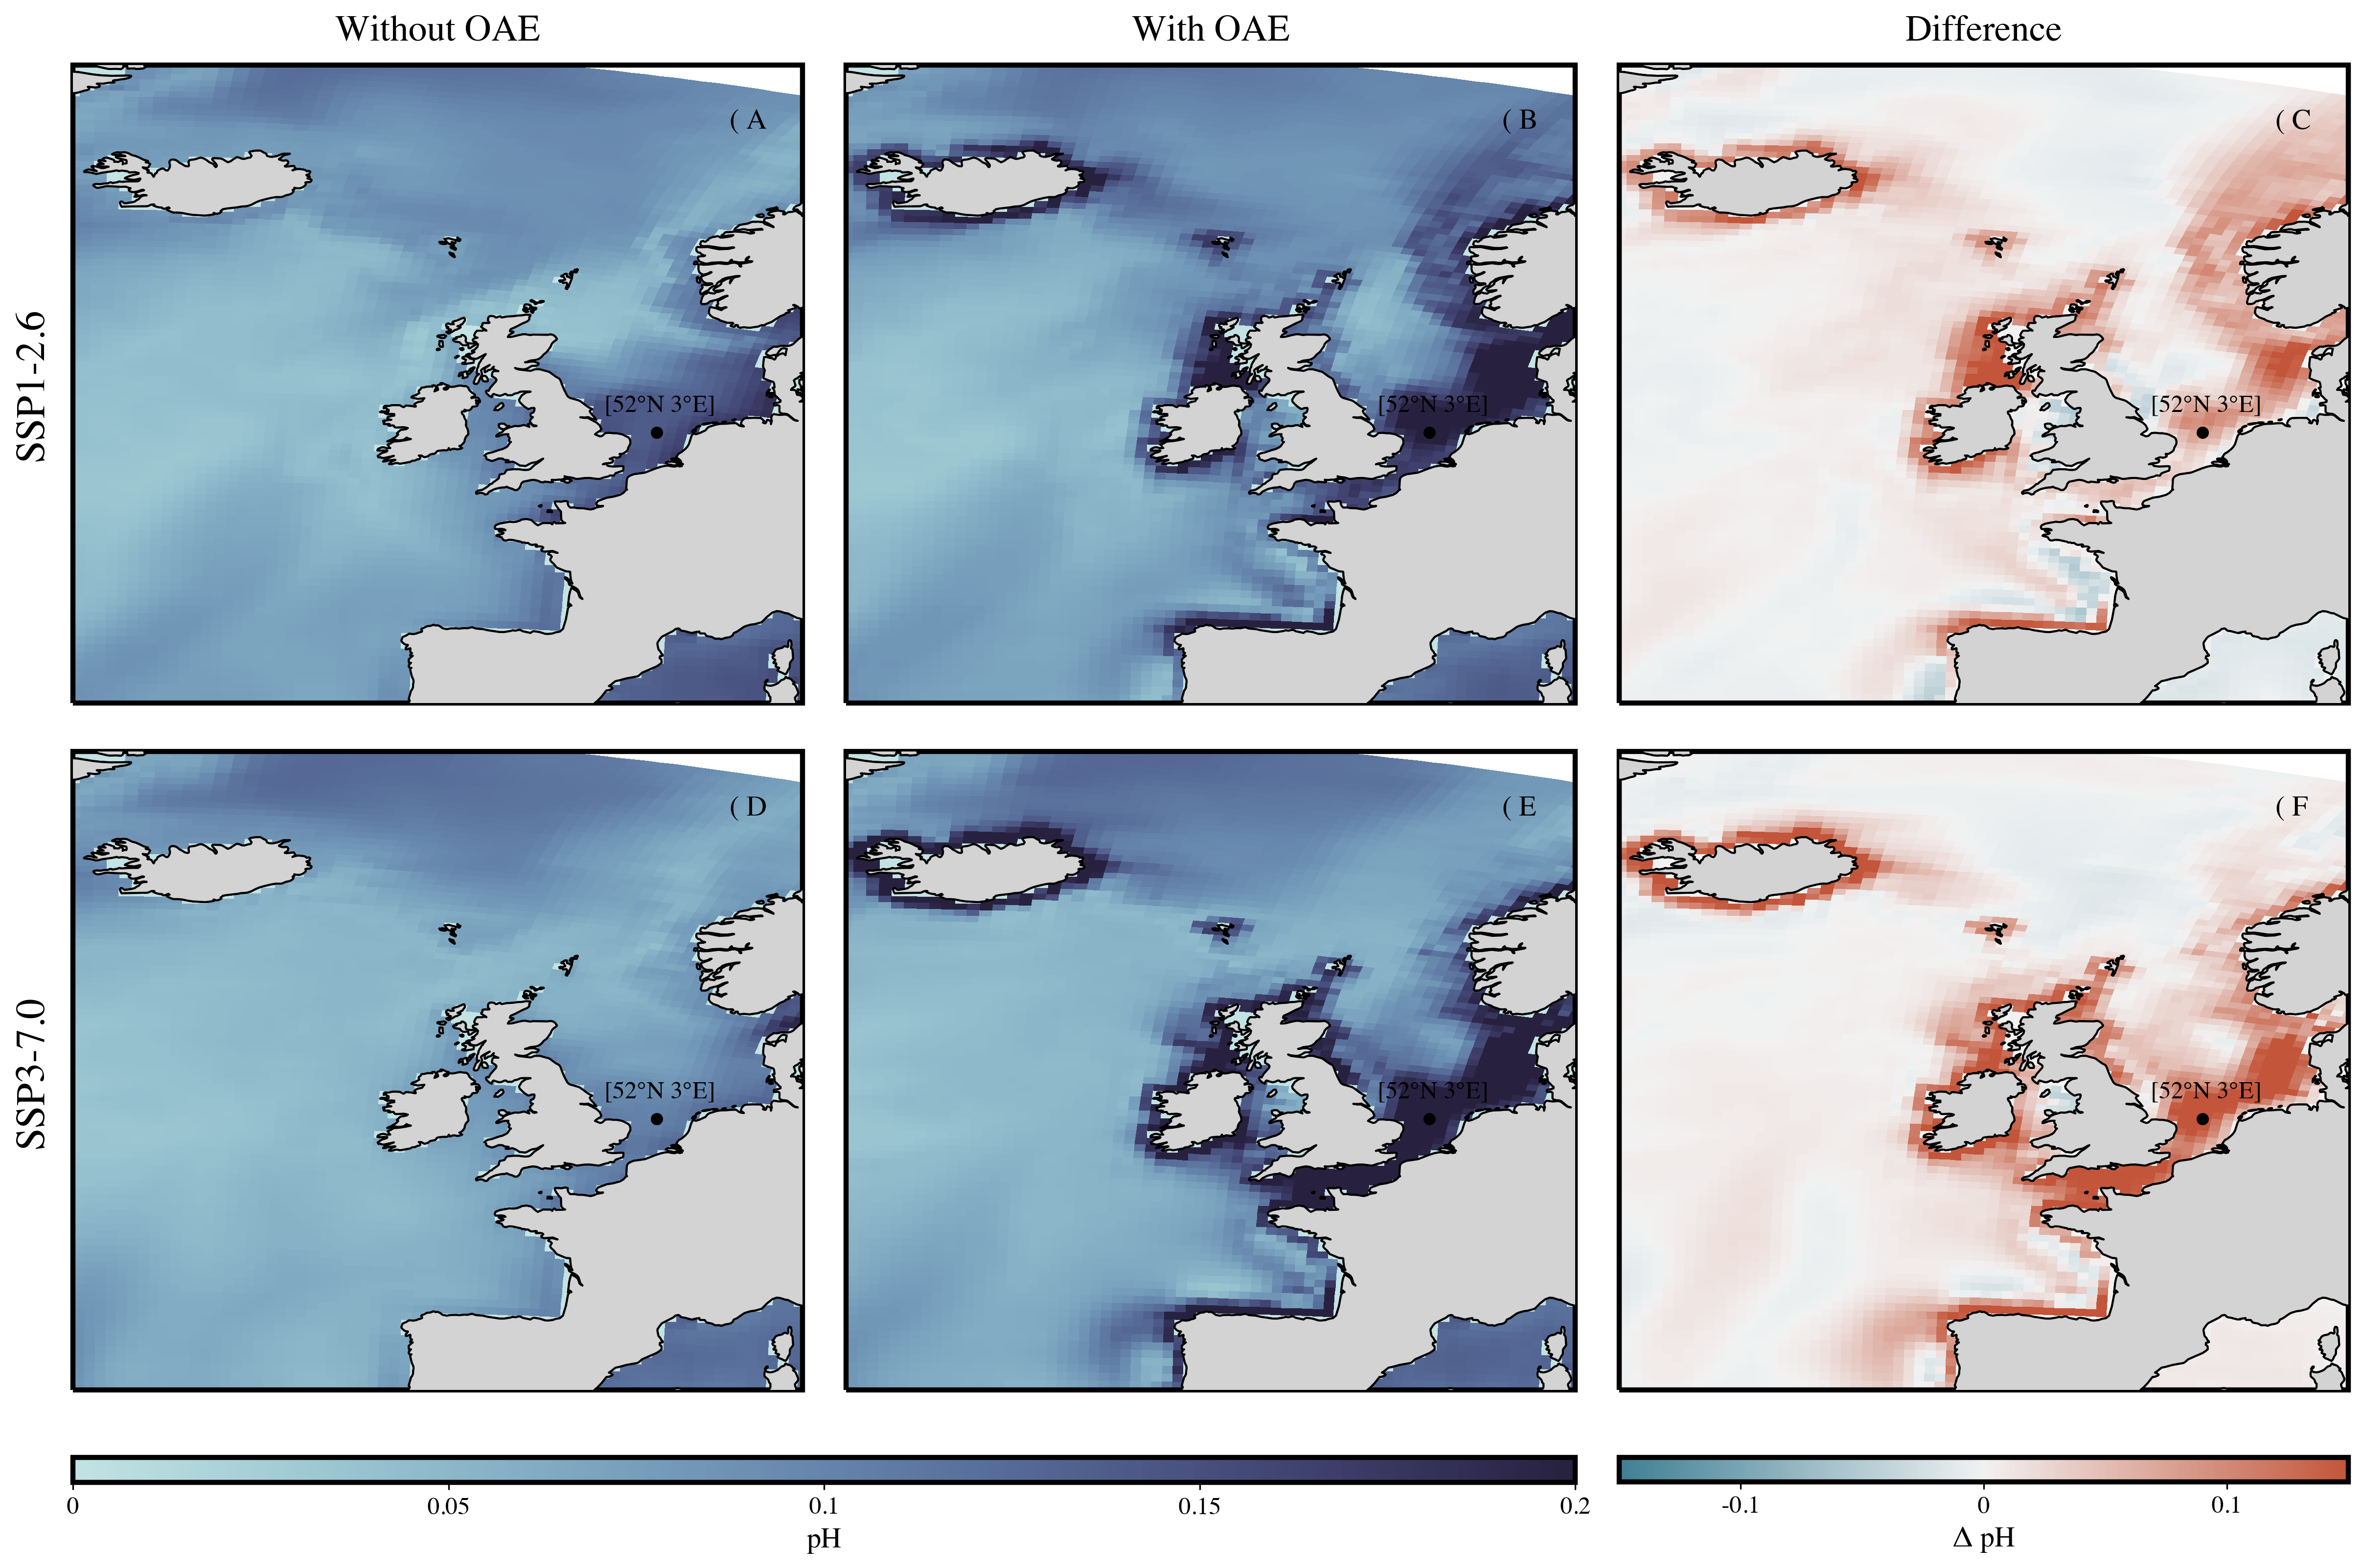
\includegraphics[width=15cm]{fig/3_Results/pH/ph_ampl.png}

\end{figure}

Modifications to the pH amplitude are not geographically homogeneous in SSP1-2.6 (top row in \cref{phamplitude}). In most of the European regions, pH seasonality expands, whereas a flattening is detected in the southern UK, western France and Spain (blue regions in C of \cref{phamplitude}). All changes are constrained to the vicinity of the coastline, where alkalinity addition was simulated. Under a higher-warming scenario, the pH seasonal amplitude cycle is better defined, showing that the entire European shore undergoes a strong increase in amplitude (red regions in F of \cref{phamplitude}). In both scenarios at open ocean, signals are mild or absent. 

\section[\texorpdfstring{DIC}{DIC}]{\ac{dic}:}

\begin{figure}[H]
\caption[Monthly average of baseline and \texorpdfstring{OAE}{OAE}-induced \texorpdfstring{DIC}{DIC}]{From left to right, monthly average of baseline and \ac{oae}-induced \ac{dic} (mmol m\textsuperscript{-3}) in the European region in SSP1-2.6 (A), and in SSP3-7.0 (C), and at location S in SSP1-2.6 (E) and in SSP3-7.0 (G) averaged over 2090-2100 (top), and the difference ($\Delta$) (B, D, F, and H) between the two scenarios (bottom).}
\label{dic}
\centering
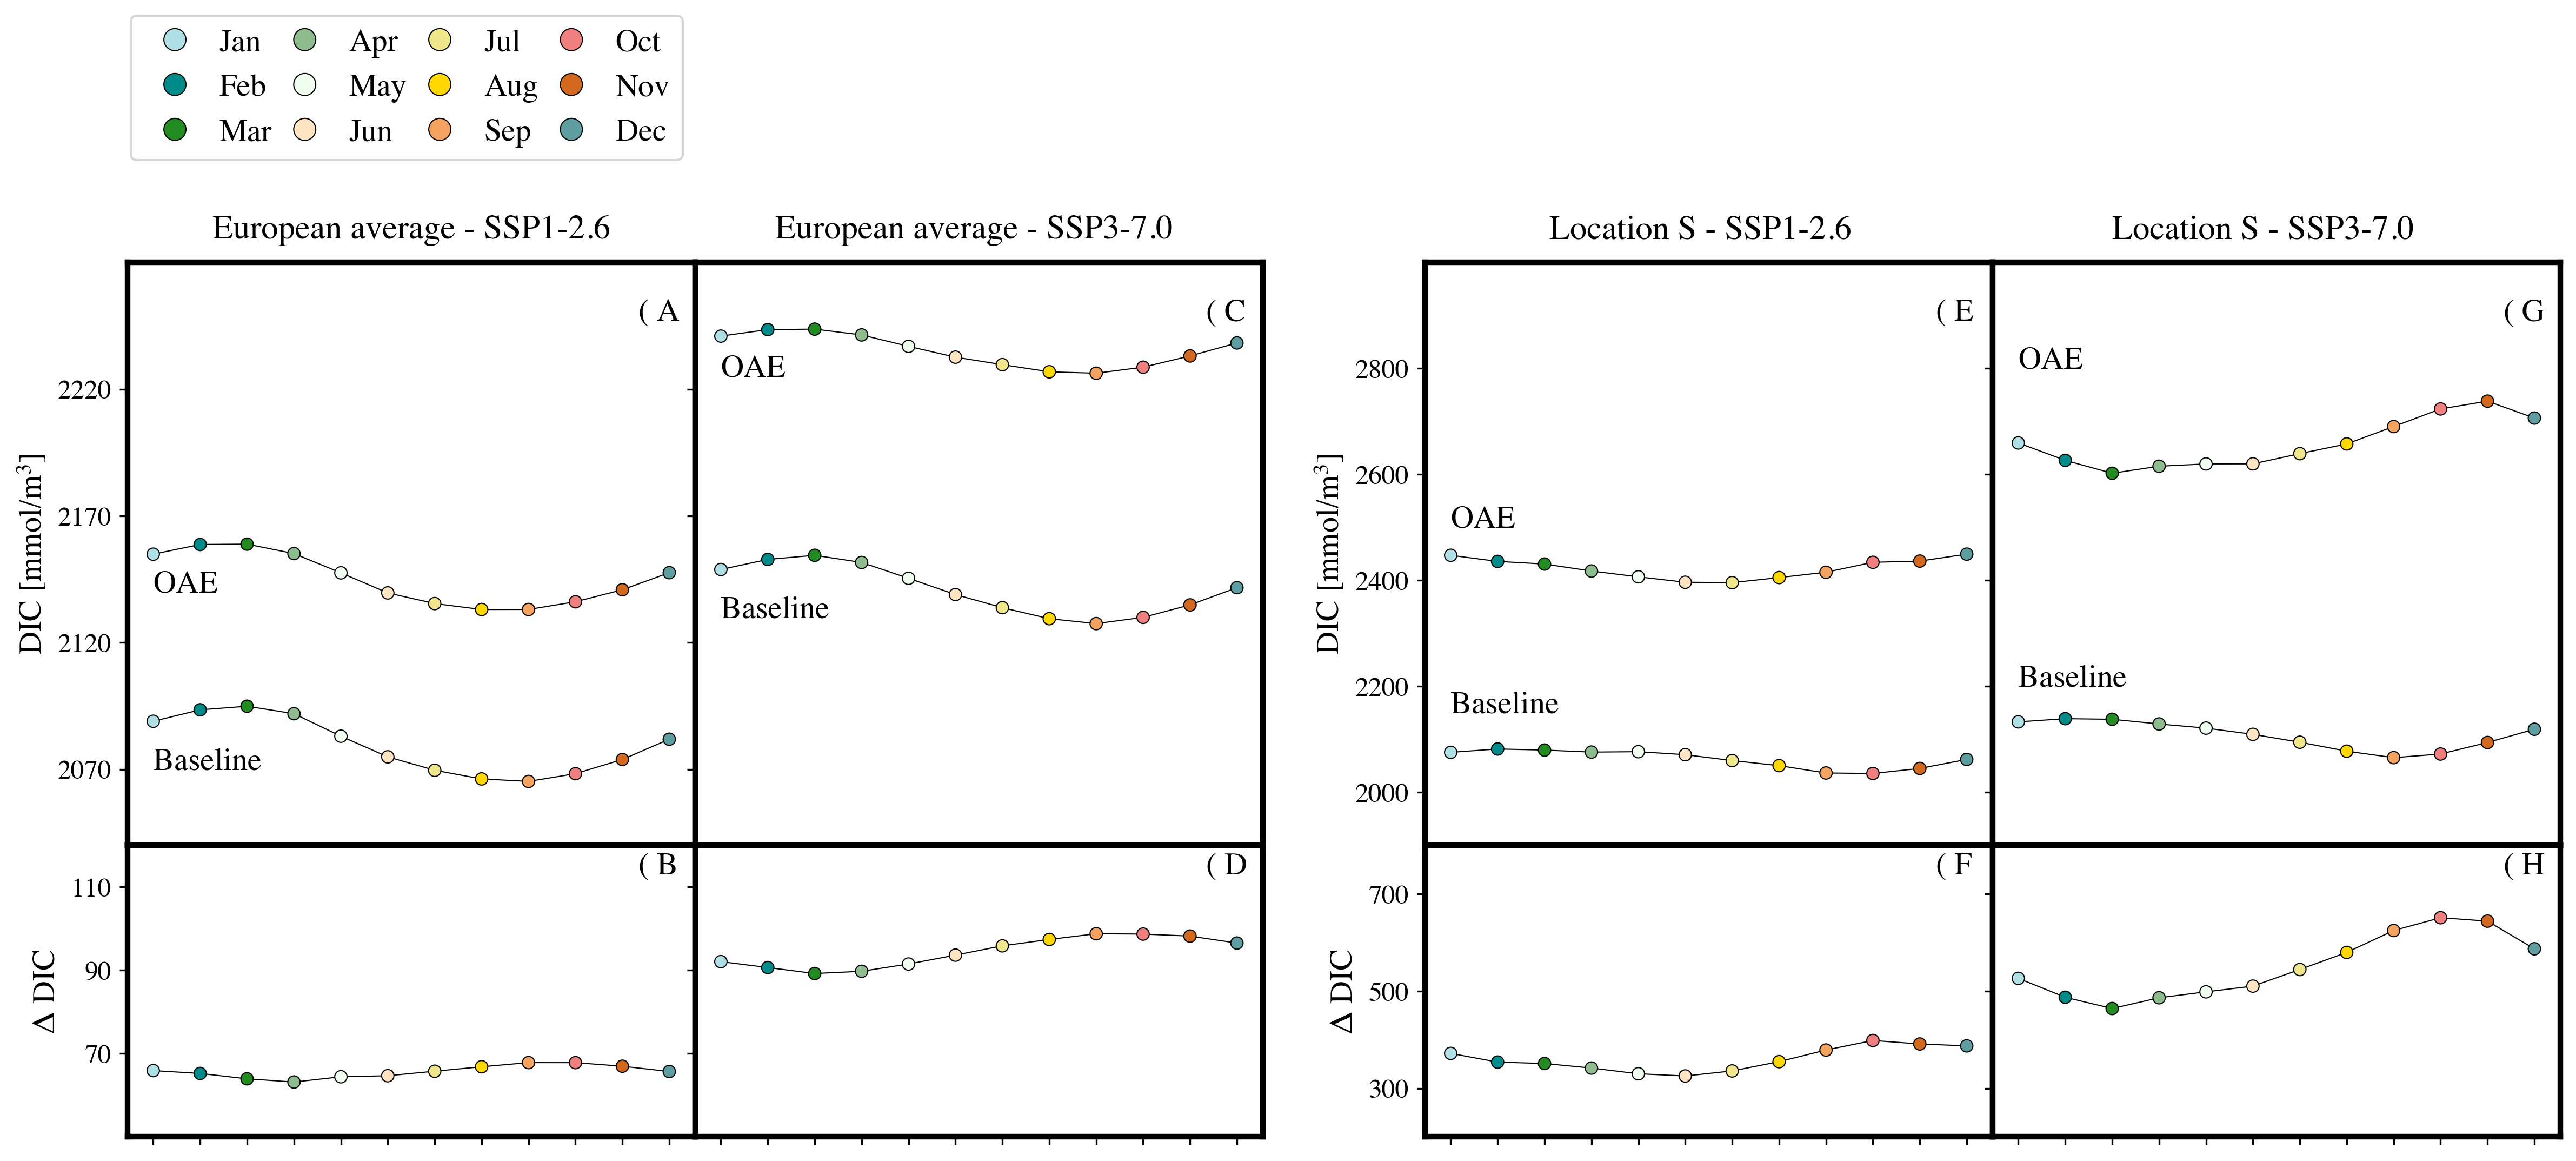
\includegraphics[width=15cm]{fig/3_Results/DIC/dic.png}

\end{figure}

In the European region in SSP1-2.6, \ac{dic} is characterised by highest and lowest levels in March and September, respectively. The average \ac{dic} seasonal cycle spans from 2065 to 2095 mmol m\textsuperscript{-3}. With \ac{oae} application, the \ac{dic} pool is significantly enhanced due to more \ch{CO2} input into the ocean but keeps reproducing the same seasonal pattern as the baseline. As for the amplitude, although minimal, a compression of 4 mmol m\textsuperscript{-3} is registered. Signal anomalies between scenarios are mainly detected between in autumn. In SSP3-7.0, \ac{dic} absolute values increase in response to rising atmospheric \ch{CO2} concentrations and consequent higher \ch{CO2} input into the ocean. D of \cref{dic} reveals that \ac{oae} is more efficient in driving \ac{dic} replenishment. 

At location S in SSP1-2.6, the ocean surface \ac{dic} is highest over the winter months and lowest in autumn. With \ac{oae}, minima are anticipated to the beginning of summer. The \ac{oae}-induced seasonal cycle stretches from 2396 to 2450 mmol m\textsuperscript{-3}. In SSP3-7.0, \ac{oae} forces the system to a shift. Carbon content increases at the ocean surface in November whereas undersaturation takes place especially in March, where the curve begins rising again. This describes a meaningful seasonal alteration from the baseline. The current cycle spans from 2602 to 2738 mmol m\textsuperscript{-3}. Both $\Delta$ \ac{dic} of SSP3-7.0 (D and H of \cref{dic}) show a larger baseline-to-\ac{oae} anomaly than their respective SSP1-2.6.

\begin{figure}[H]
\caption[\texorpdfstring{DIC}{DIC} seasonal amplitude change]{\ac{dic} seasonal amplitude change (mmol m\textsuperscript{-3}) without \ac{oae} (left), with \ac{oae} (middle), and the difference ($\Delta$) between the two (right). SSP1-2.6 (top) and SSP3-7.0 (bottom).}
\label{dicamplitude}
\centering
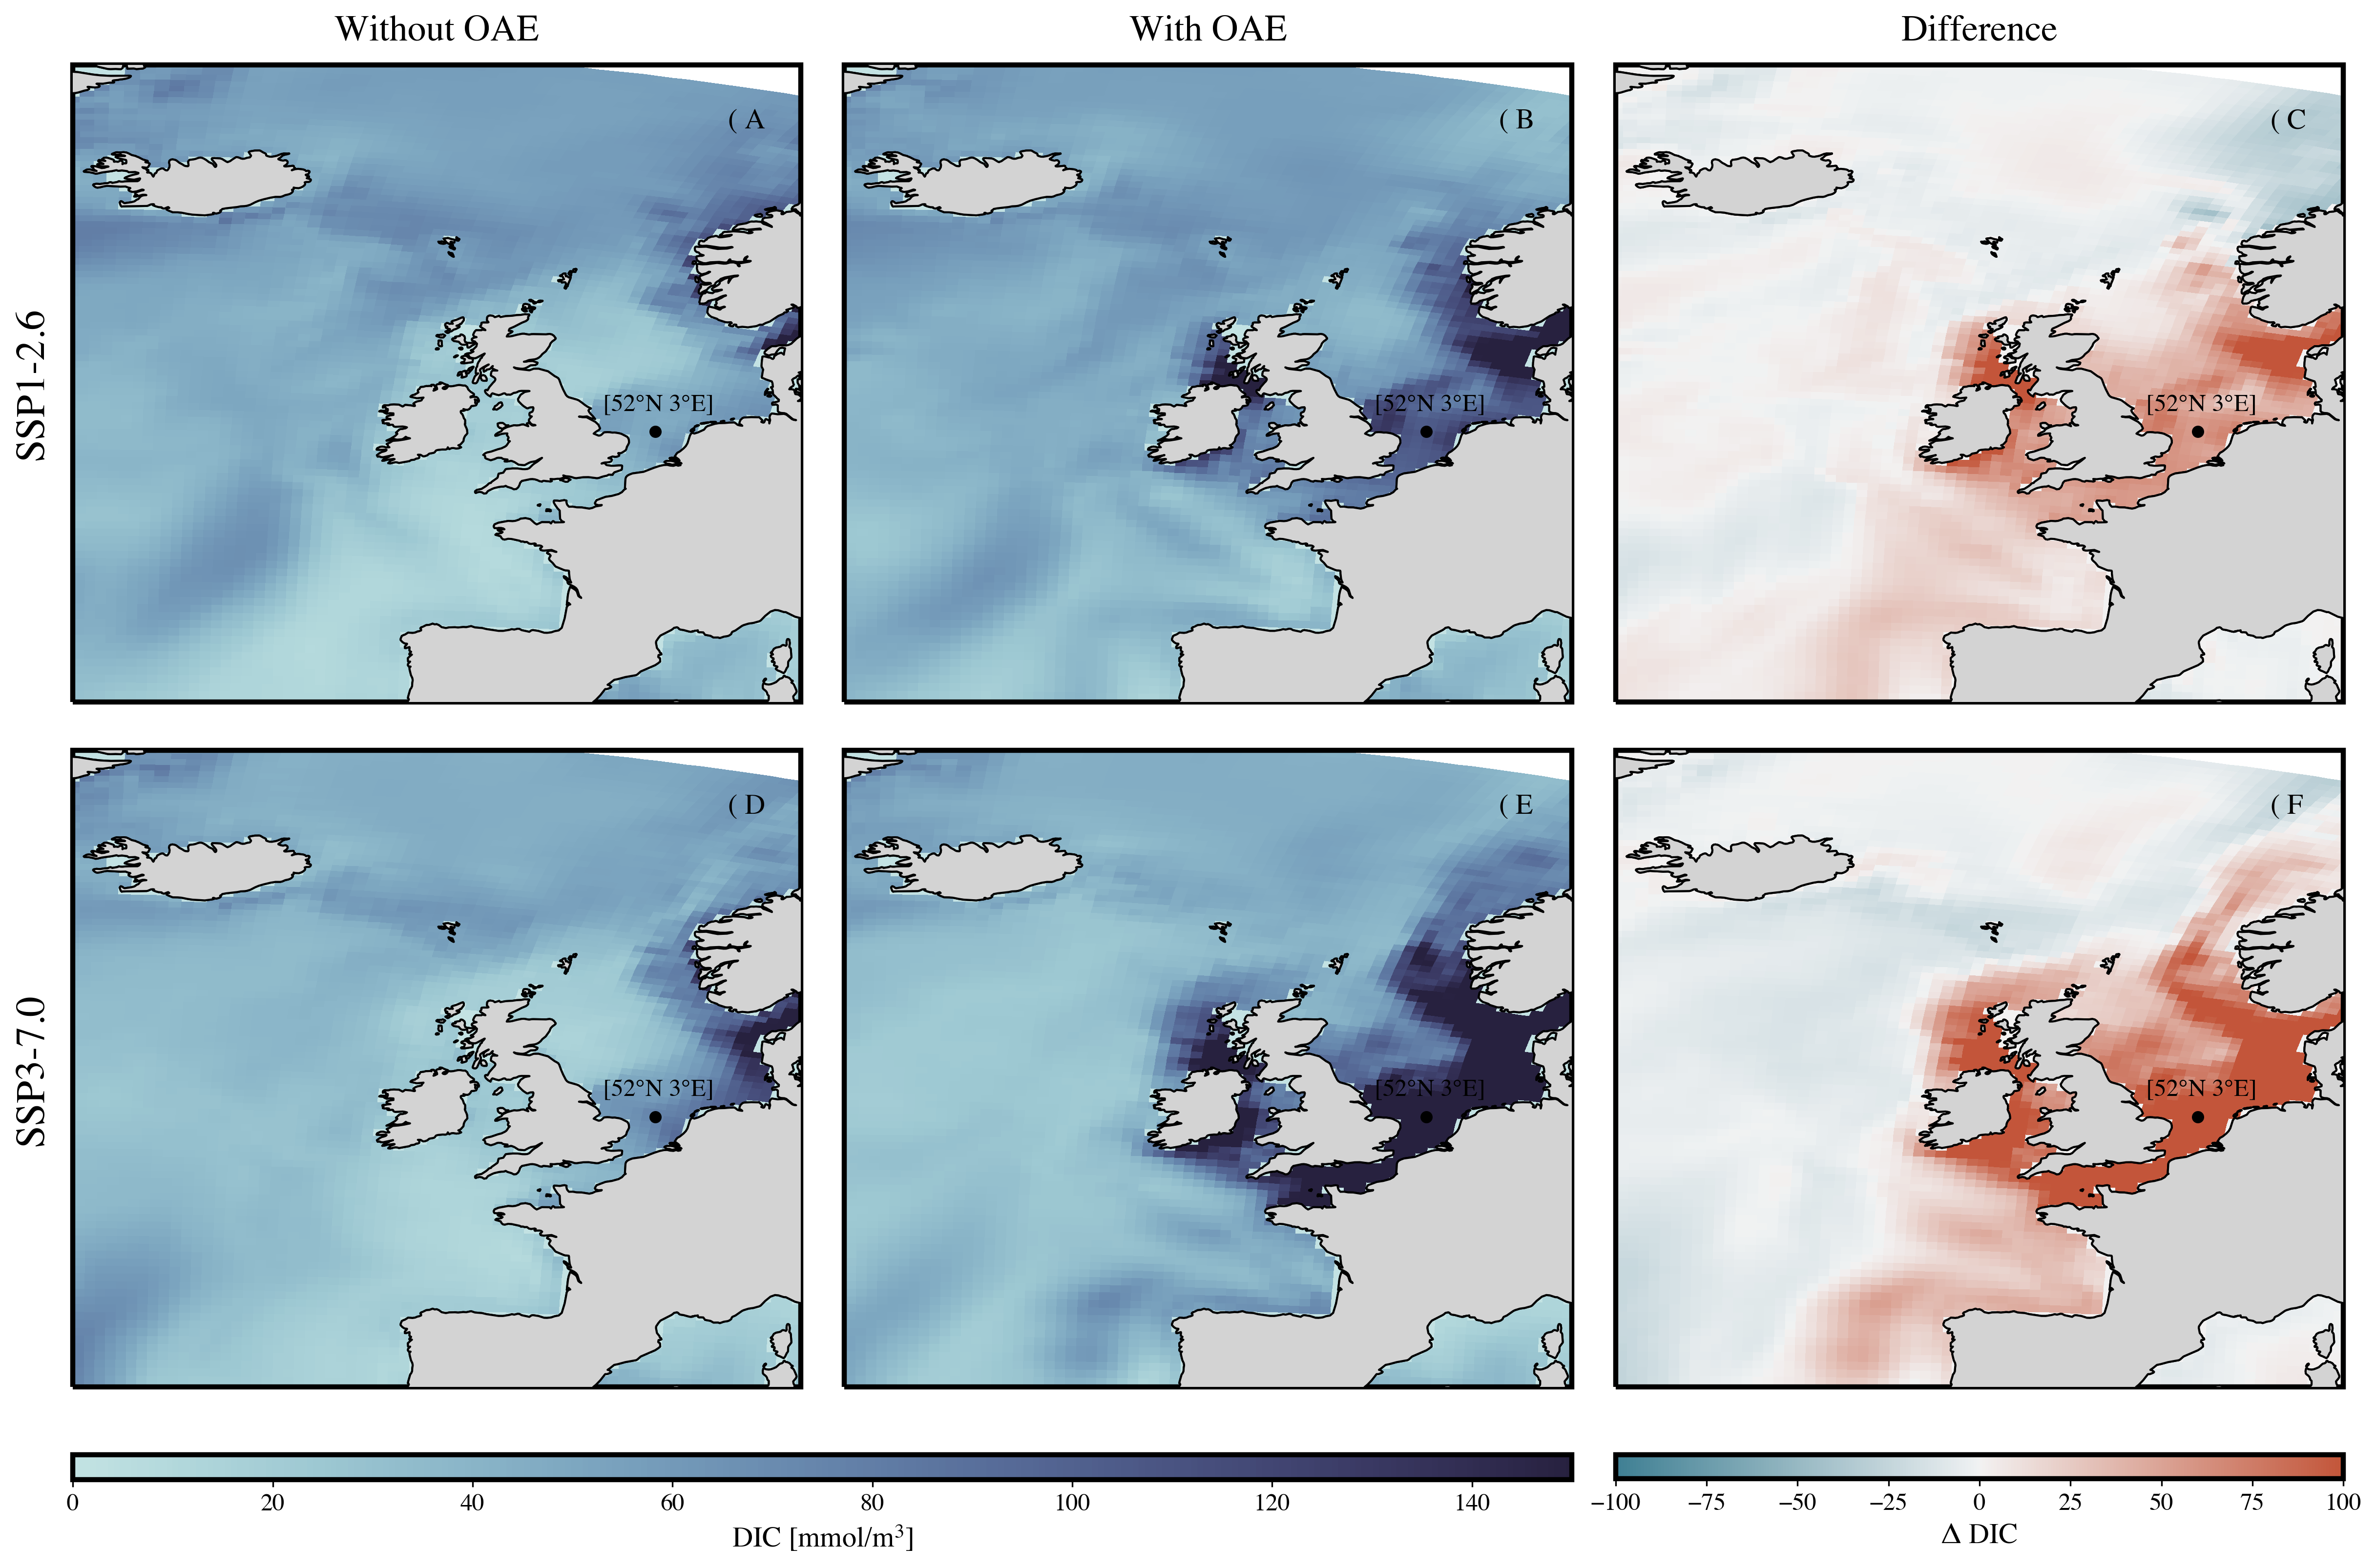
\includegraphics[width=15cm]{fig/3_Results/DIC/dic_amplitude.png}

\end{figure}

In SSP1-2.6, the most pronounced \ac{dic} seasonal amplification is observed only at two locations: off of the coasts of northern Northern Ireland and in the Skagerrak sea (dark red regions in C of \cref{dicamplitude}). A less acute seasonal amplification is still detected in the southern and central North Sea whereas, at open ocean, no propagation occurs and most regions remain overall unaffected. In SSP3-7.0, the \ac{dic} seasonal cycle is much more amplified with respect to the baseline, although confined to the partly enclosed North Sea and the UK coastline. Mild amplification is observed by the Spanish and Norwegian banks. 

\section{Ocean \ch{pCO2}:}

\begin{figure}[H]
\caption[Monthly average of baseline and \texorpdfstring{OAE}{OAE}-induced ocean \ch{pCO2}]{From left to right, monthly average of baseline and \ac{oae}-induced ocean \ch{pCO2} (µatm) in the European region in SSP1-2.6 (A), and in SSP3-7.0 (C), and at location S in SSP1-2.6 (E) and in SSP3-7.0 (G) averaged over 2090-2100 (top), and the difference ($\Delta$) (B, D, F, and H) between the two scenarios (bottom).}
\label{fco2}
\centering
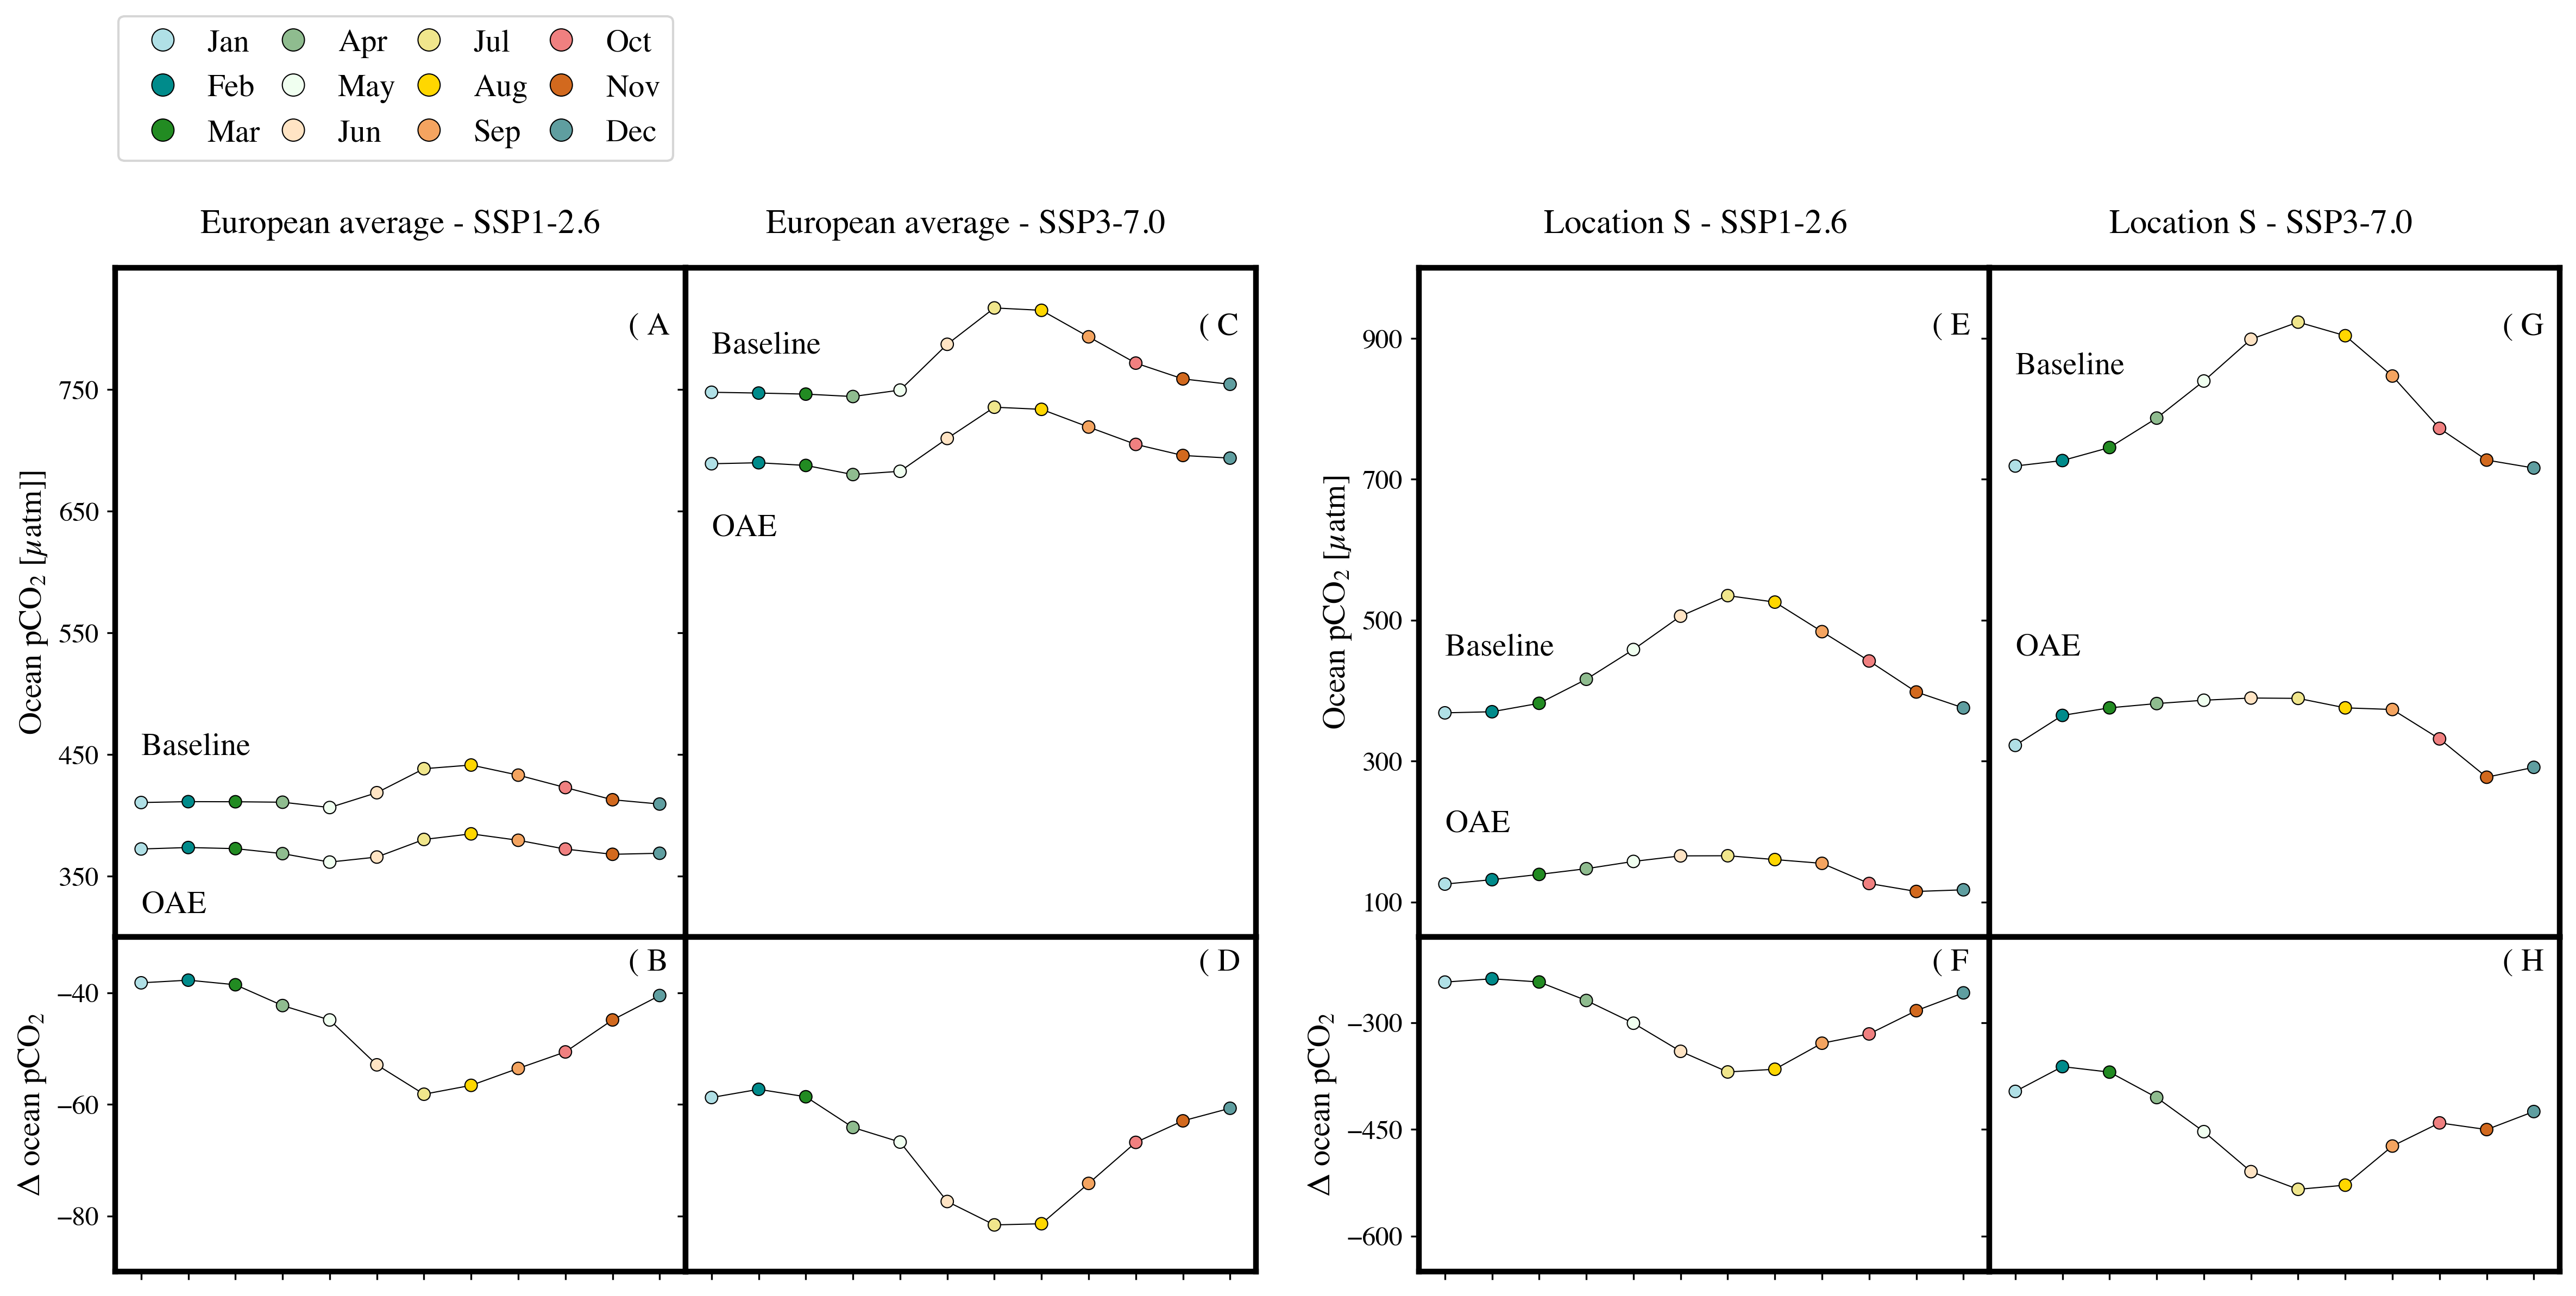
\includegraphics[width=15cm]{fig/3_Results/pCO2/fco2.png}

\end{figure}

In the European region in SSP1-2.6, ocean \ch{pCO2} is characterised by least and most elevated values in May and August, respectively, with a mean amplitude stretching from 407 to 441 µatm. In the \ac{oae} scenario, \ch{CO2} partial pressure is reduced due to alkalinity enhancement and \ch{pCO2} absolute values drop, now spanning between 362 and 385 µatm. The seasonal amplitude of the \ac{oae} scenario is therefore depressed. $\Delta$ \ch{pCO2} detects the largest anomalies between the two scenarios in summer (B of \cref{fco2}), signifying that alkalinity encourages \ch{pCO2} decline when \ch{CO2} outgassing takes place. In SSP3-7.0 baseline, \ch{pCO2} maintains an ascending trend until 2100 (not shown). Seasonally, elevated values are recorded in July and then decline until minima are reached in April. The mean seasonality has highest and lowest peaks of 817 and 744 µatm, respectively. In C of \cref{fco2}, it is evident that \ac{oae} induces the cycle to decrease substantially, with an amplitude of 55 µatm. 

Unlike the European average, location S displays minima in winter, denoting that \ch{pCO2} decrease is here anticipated. Predictably, \ac{oae} reduces \ch{pCO2} absolute values. The seasonal amplitude is compressed to less than a third compared to the baseline, with an average span of 51 µatm. $\Delta$ \ch{pCO2} oscillates between winter lows and summer highs, as \ac{oae} primarily helps to weaken the ocean pressure that encourages \ch{CO2} to escape. In SSP3-7.0, the baseline has a seasonal amplitude ranging between 716 and 923 µatm. Alkalinity addition causes \ch{pCO2} to drop substantially. Its seasonal cycle is also compressed and stays between 277 and 390 µatm. $\Delta$ \ch{pCO2} confirms that the largest discrepancy takes place in summer, at highest ocean \ch{pCO2} (H of \cref{fco2}). 

\begin{figure}[H]
\caption[\ch{pCO2} seasonal amplitude change]{\ch{pCO2} seasonal amplitude change (µatm) without \ac{oae} (left), with \ac{oae} (middle), and the difference ($\Delta$) between the two (right). SSP1-2.6 (top) and SSP3-7.0 (bottom).}
\label{pco2amplitude}
\centering
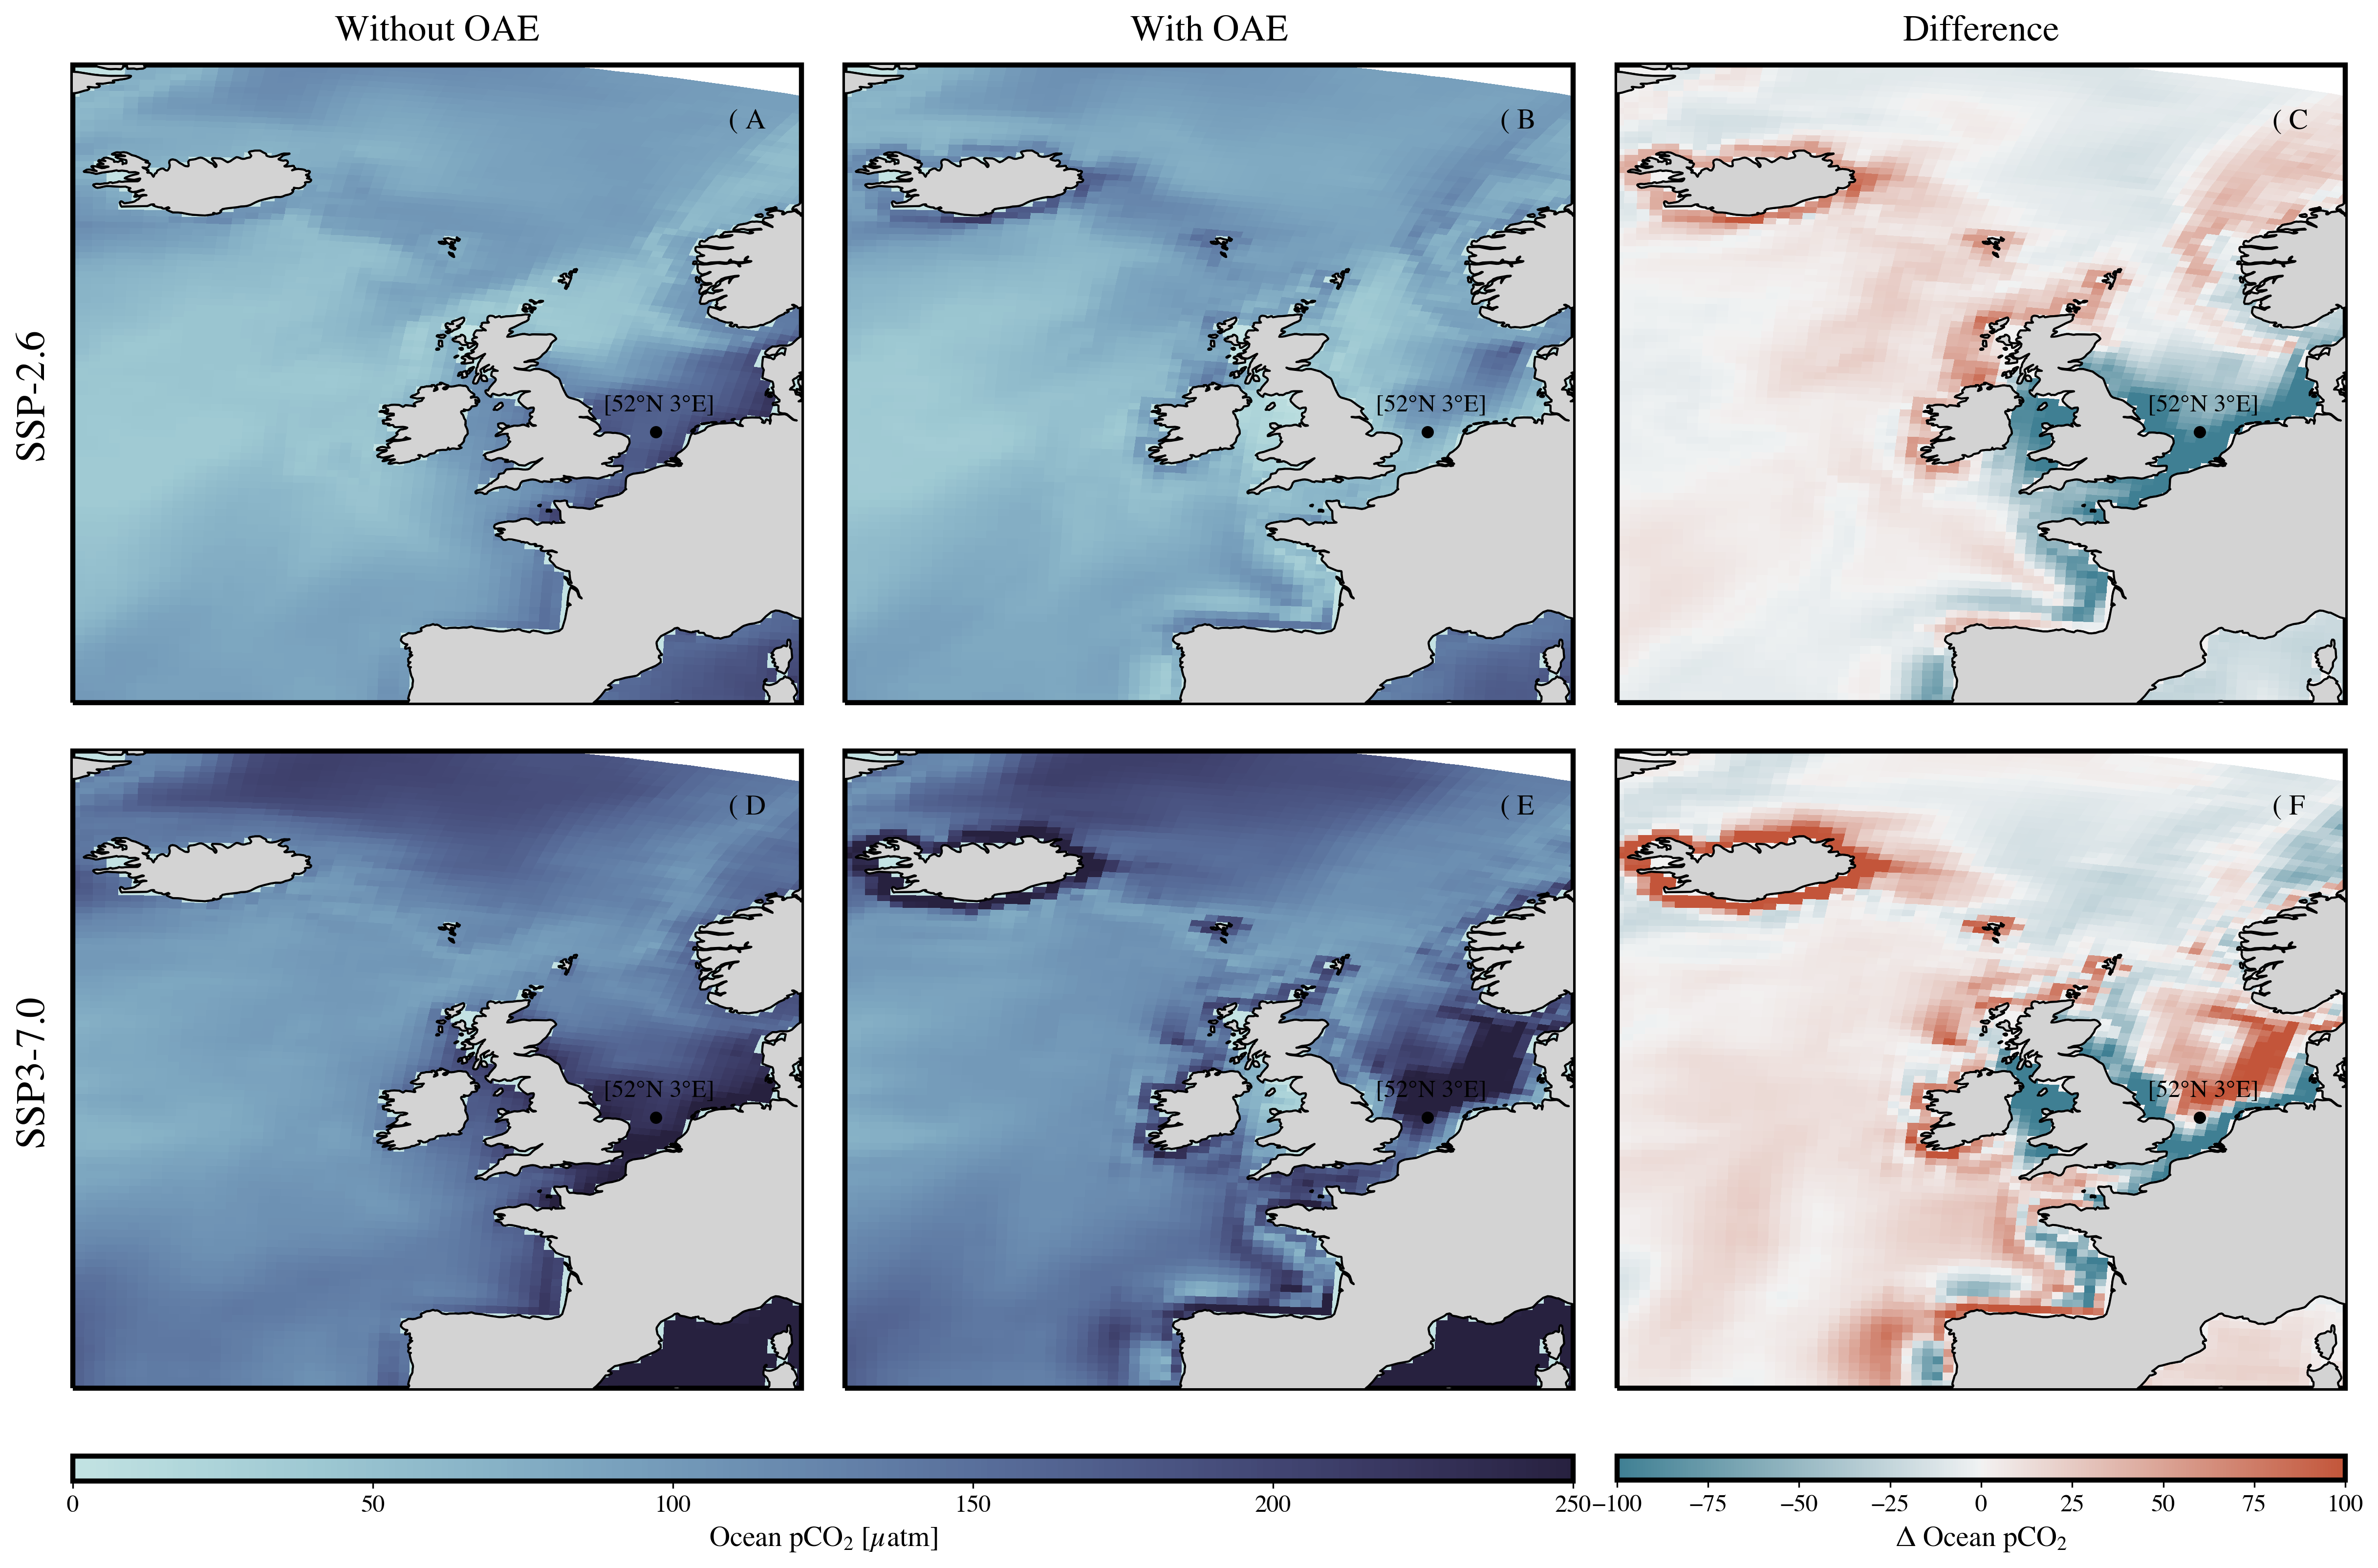
\includegraphics[width=15cm]{fig/3_Results/pCO2/fco2_ampl.png}

\end{figure}

In \cref{pco2amplitude} for SSP1-2.6, a clear pattern is identified at the proximity of the injection location, with two diverging geographies. At higher latitudes, in Iceland, the Norwegian, the Spanish North and the British North-West bank, \ch{pCO2} seasonal amplitude is slightly more pronounced than the baseline (red regions in C of \ref{pco2amplitude}). Conversely, at lower latitudes including the mainland shore and the central-to-southern UK coasts, \ch{pCO2} seasonal breadth is strongly mitigated (blue regions). In SSP3-7.0, \ch{pCO2} amplitude behaves similarly, with the exception of the centre-to-north North Sea and northern Spain, where strong amplification is displayed. At open sea, \ch{pCO2} seasonality is slightly amplified in the North Atlantic and dampened in the sub-polar regions.

\section{\ch{CO2} flux:}

\begin{figure}[H]
\caption[Monthly average of baseline and \texorpdfstring{OAE}{OAE}-induced ocean \ch{CO2} flux]{From left to right, monthly average of baseline and \ac{oae}-induced ocean \ch{CO2} (mmol/m\textsuperscript{2}/yr) in the European region in SSP1-2.6 (A), and in SSP3-7.0 (C), and at location S in SSP1-2.6 (E) and in SSP3-7.0 (G) averaged over 2090-2100 (top), and the difference ($\Delta$) (B, D, F, and H) between the two scenarios (bottom). Negative values represent \ch{CO2} uptake by the ocean.}
\label{co2flux}
\centering
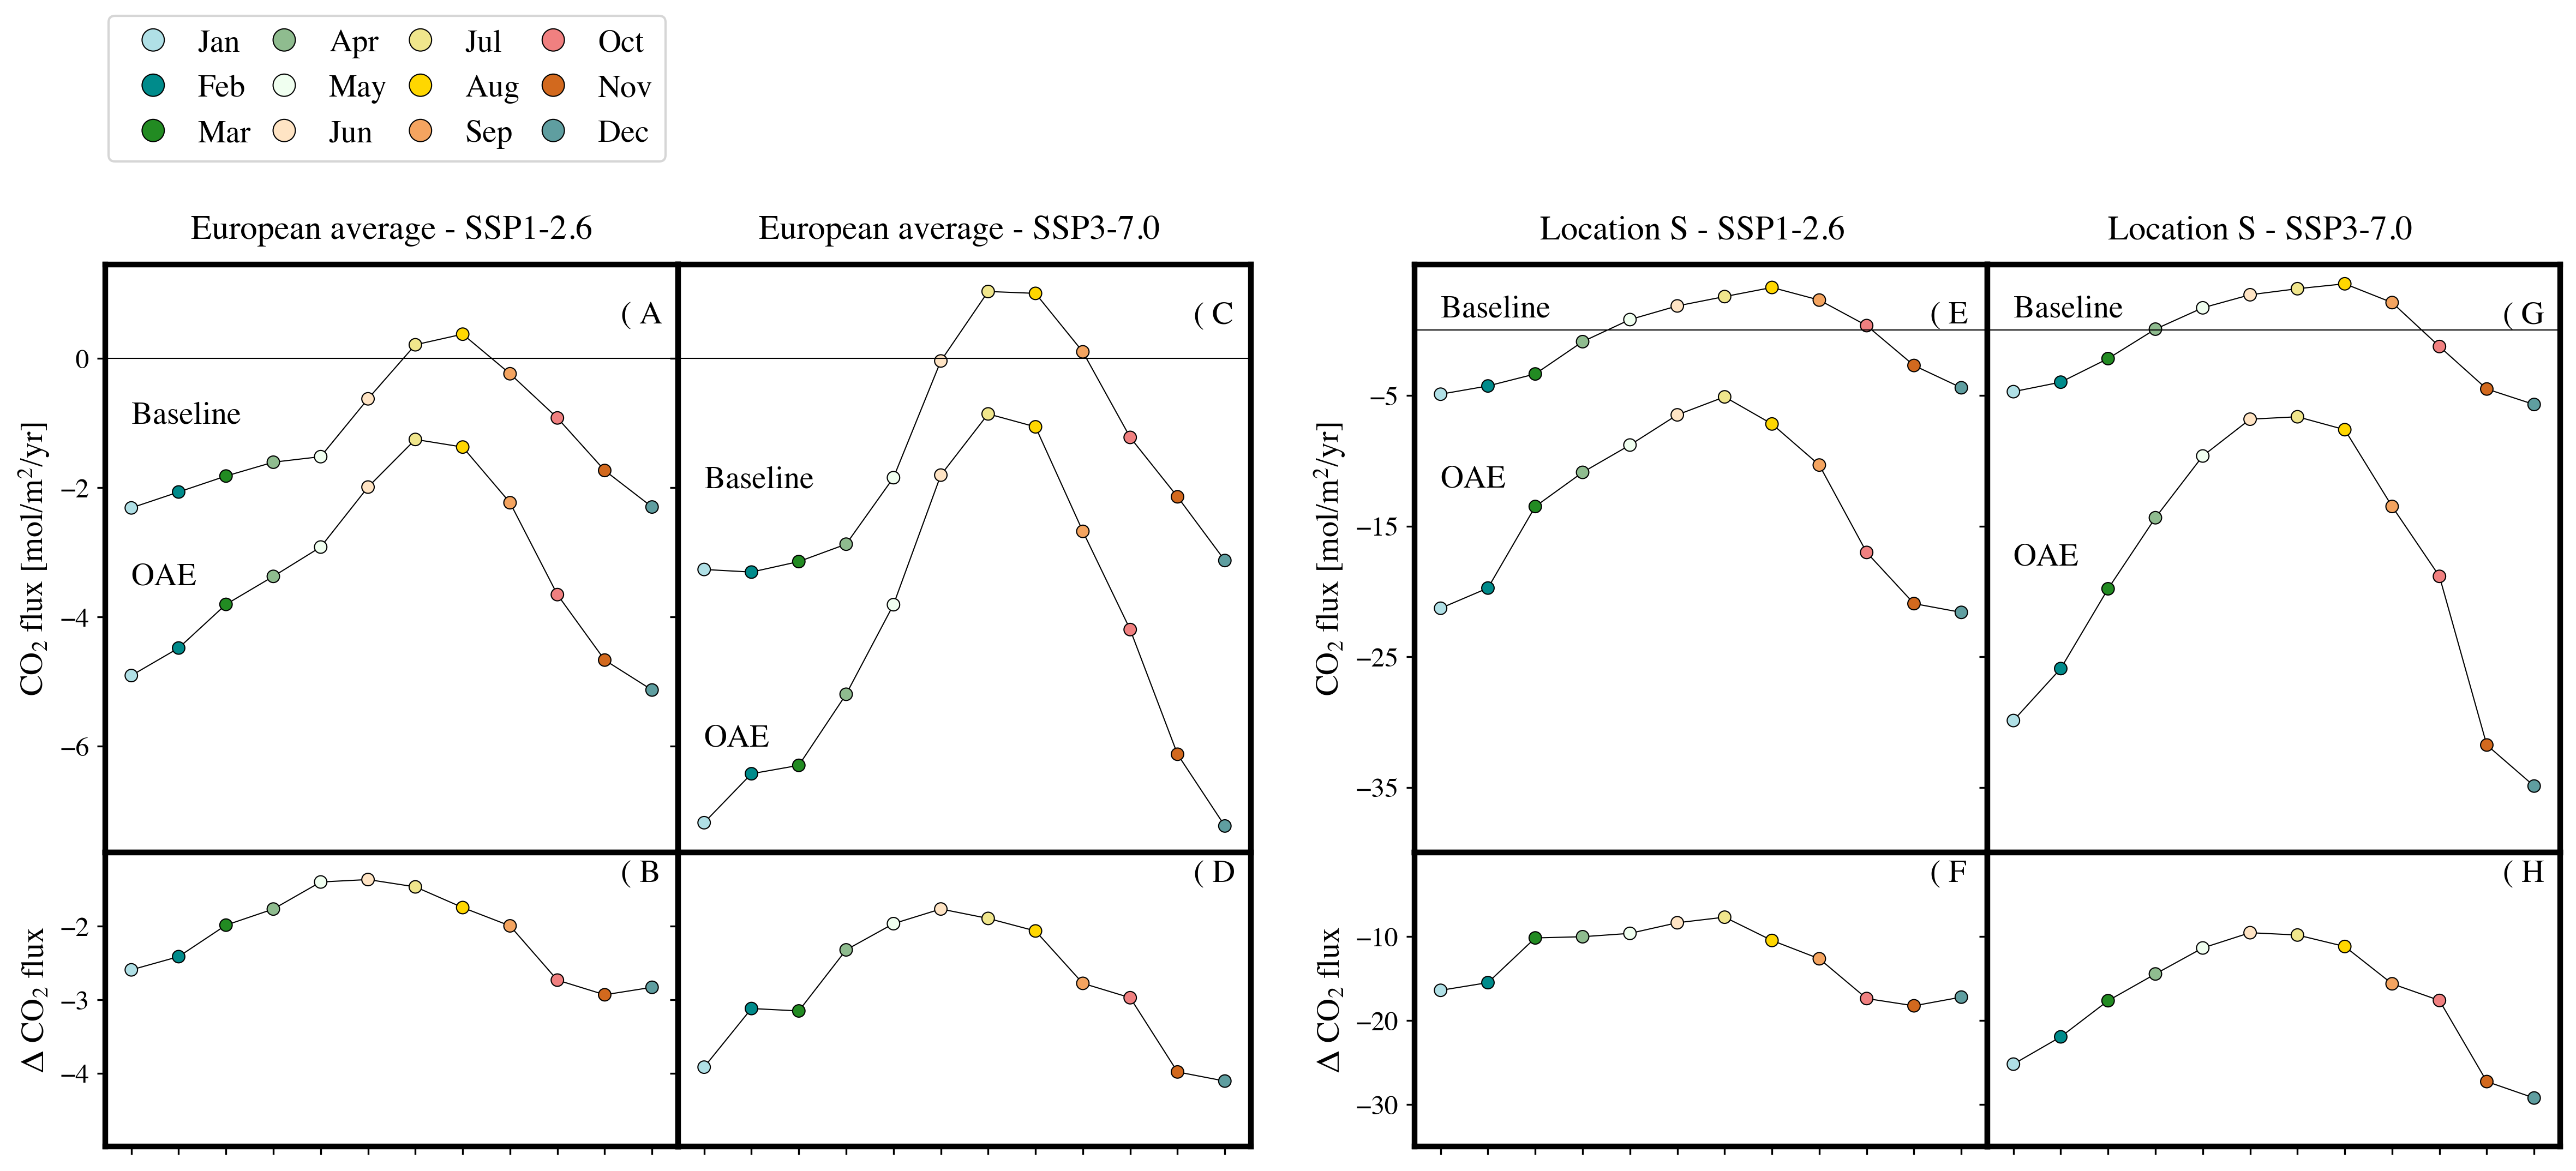
\includegraphics[width=15cm]{fig/3_Results/CO2flux/co2flux.png}

\end{figure}

A of \cref{co2flux} shows that, at the European average in SSP1-2.6, the baseline ocean tends to outgass \ch{CO2} in summer (in July and August), while remaining a carbon sink over the rest of the year, with most pronounced uptake in winter, especially December. This outcome agrees with \ac{dic} seasonality, where winter uptake enhances the \ac{dic} pool and summer outgassing depletes it. When \ac{oae} is applied, the system is turned into a sink all year round, with summertime (wintertime) reflecting the least (most) \ch{CO2} uptake. Following the baseline, it is in July and January that extremes are detected. The seasonal amplitude varies noticeably, with the \ac{oae} scenario showing a much greater breadth than the baseline. \ch{CO2} flux amplitude has now an average span of -1.25 to -5.12, compared to the baseline that stayed between 0.37 and -2.31 mol m\textsuperscript{-2} yr\textsuperscript{-1}. In SSP3-7.0, the baseline outgasses \ch{CO2} from July to September. Adding alkalinity increases the \ch{CO2} seasonal amplitude more than the low emission scenario, especially in winter where minima $\Delta$ \ch{CO2} flux are observed. 

In the baseline of both scenarios at location S, \ch{CO2} flux reflects a downward flow in colder months and an upward flow in warmer months, splitting the annual cycle into two equally long phases. Outgassing happens from May to September/October and uptake from November to March/April, on average. In \ac{oae}-induced SSP1-2.6, \ch{CO2} flux fluctuates between -21.6 and -5.11 mol m\textsuperscript{-2} yr\textsuperscript{-1} on average, therefore doubling the baseline amplitude. Seasonality of \ch{CO2} flux in SSP3-7.0 is considerably enhanced when alkalinity is added, with a current amplitude of 28 mol m\textsuperscript{-2} yr\textsuperscript{-1}, three times larger than the baseline. In B, D, F, and H of \cref{co2flux}, the baseline-to-\ac{oae} discrepancies grow in winter and drop in summer, meaning that the impacts of alkalinisation on the ocean surface are largest when ocean uptake is already most pronounced. \ac{oae}-induced changes on the \ch{CO2} flux are disproportionately higher in winter, meaning that lower lows are not compensated for by equally higher highs.

\begin{figure}[H]
\caption[\ch{CO2} flux seasonal amplitude change]{\ch{CO2} flux seasonal amplitude change (mol m\textsuperscript{-2} yr\textsuperscript{-1}) without \ac{oae} (left), with \ac{oae} (centre), and the difference ($\Delta$) between the two (right). SSP1-2.6 (top) and SSP3-7.0 (bottom).}
\label{co2fluxamplitude}
\centering
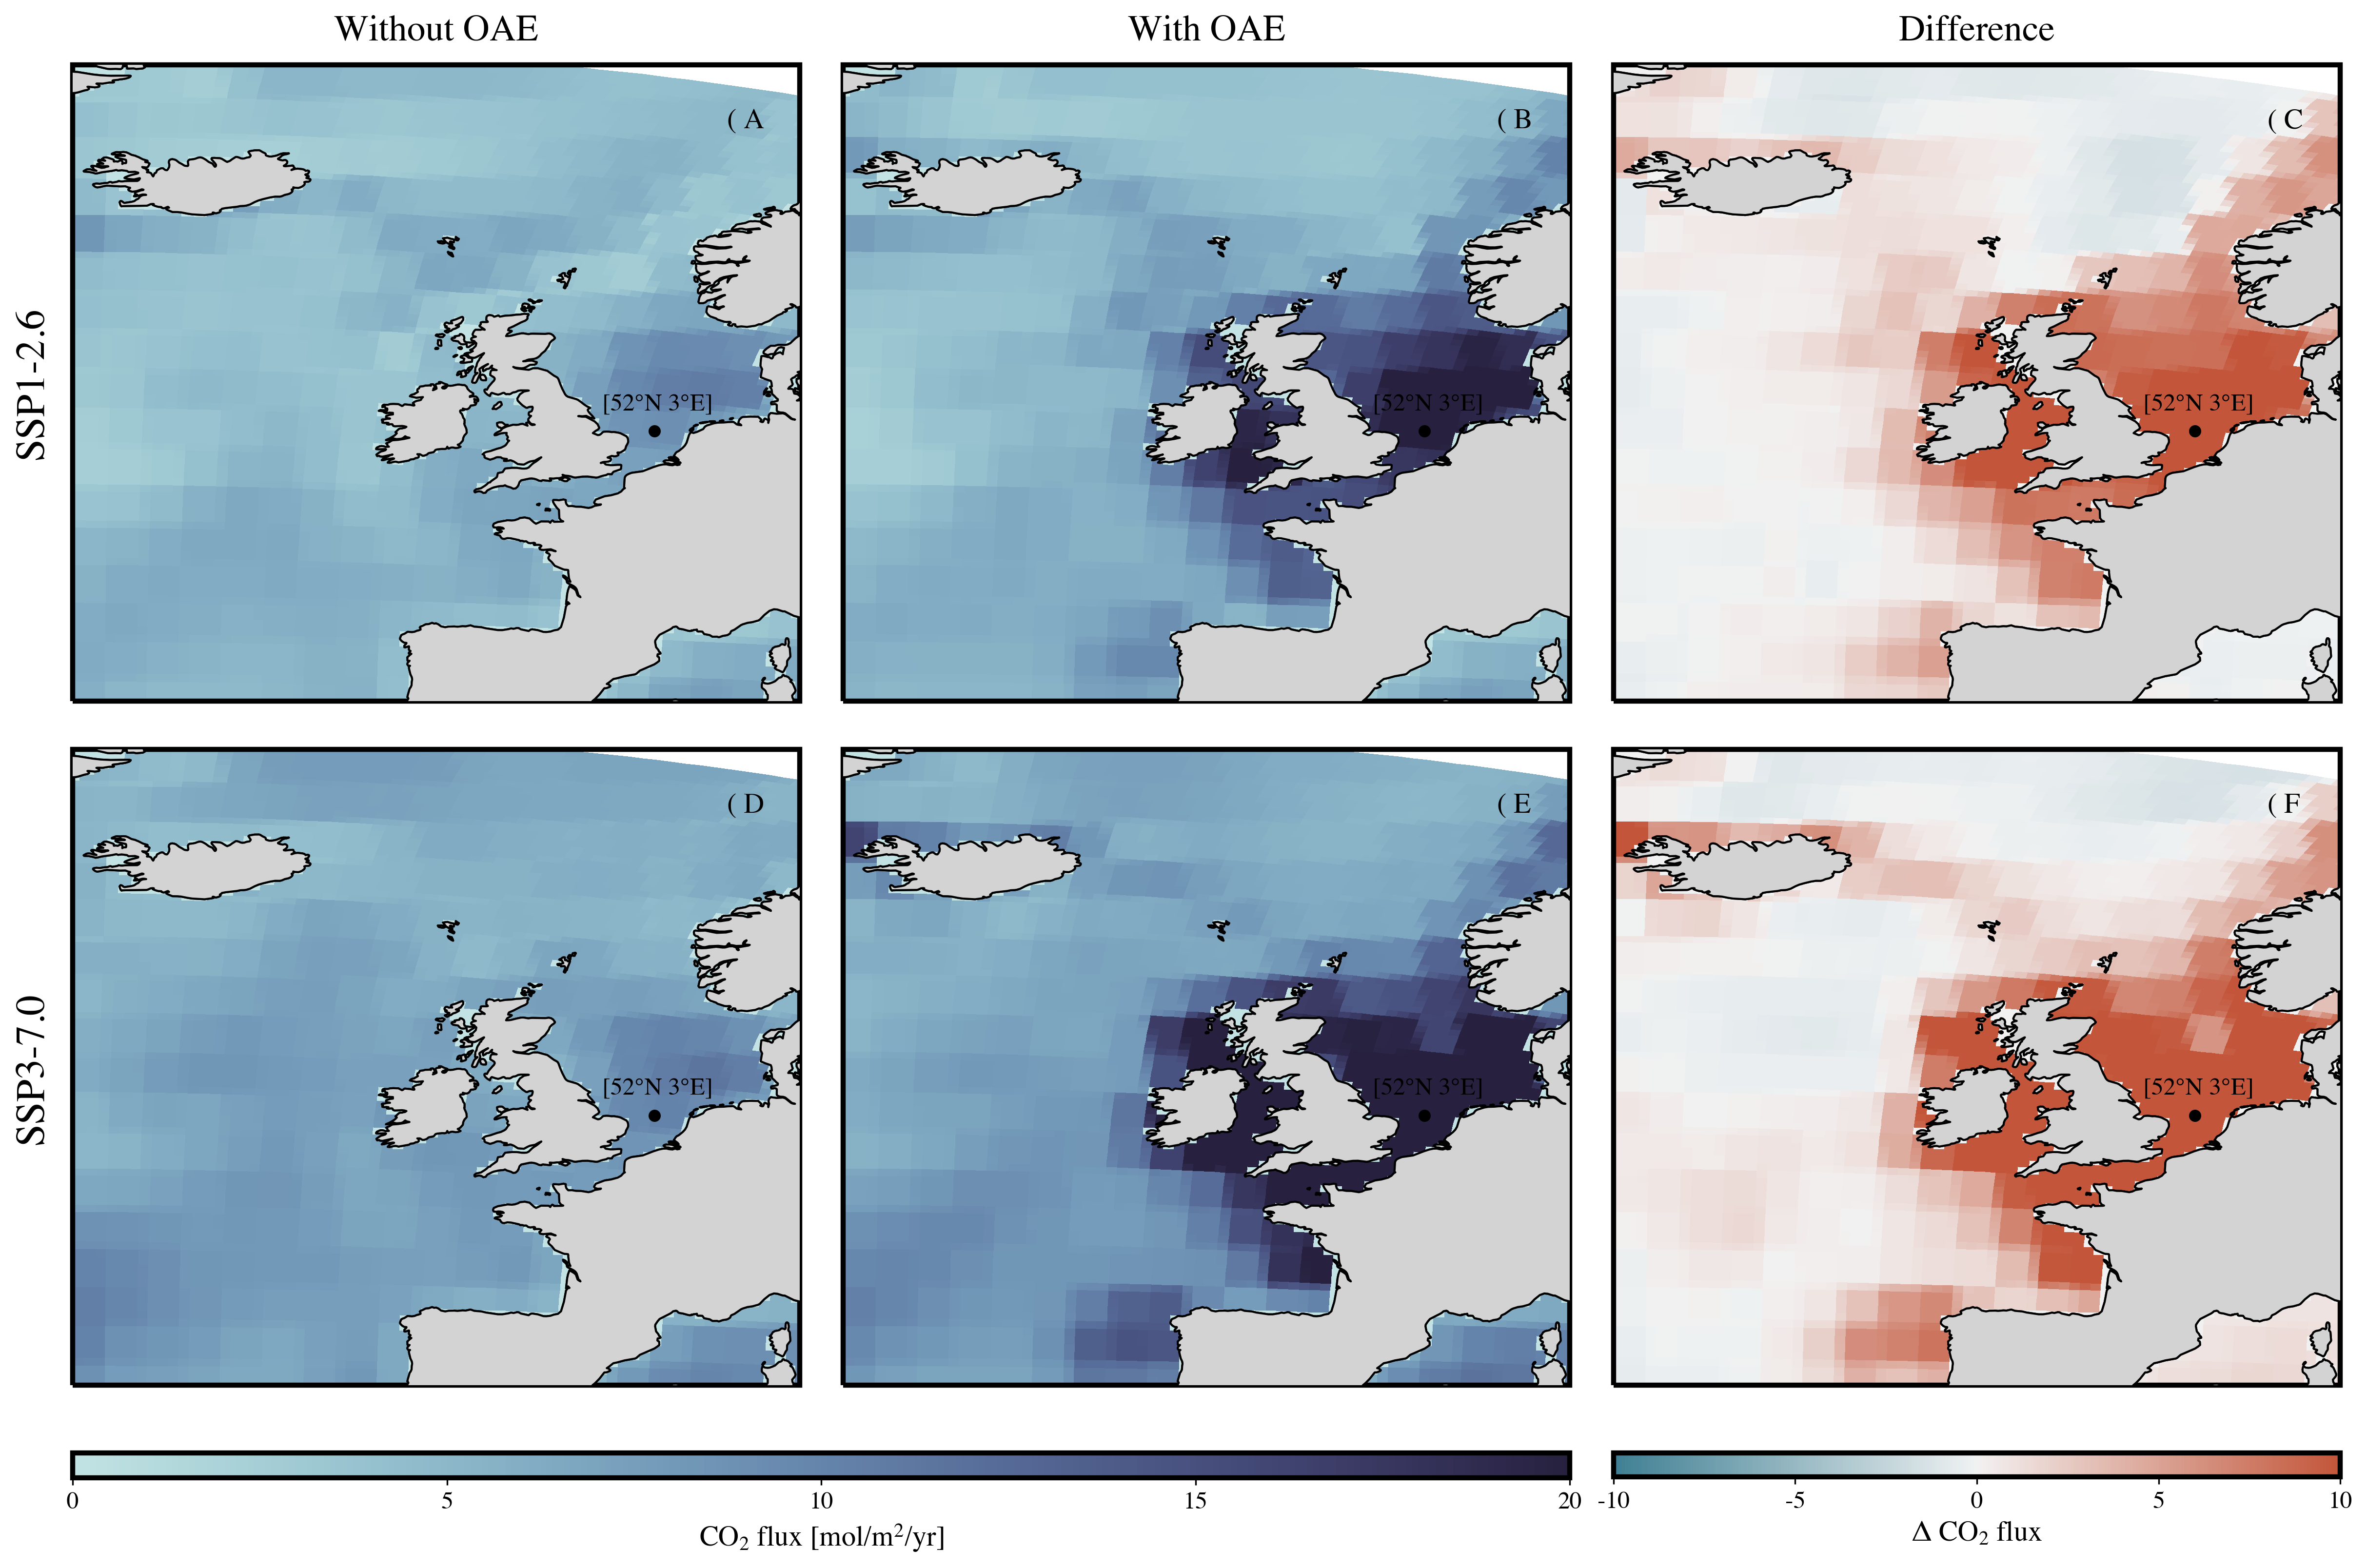
\includegraphics[width=15cm]{fig/3_Results/CO2flux/co2flux_ampl.png}

\end{figure}

With \ac{oae}, SSP1-2.6 in \cref{co2fluxamplitude} reveals an increase in \ch{CO2} seasonal fluxes along the European coasts, especially in the partially enclosed system of the southern North Sea and western UK coasts (red regions in C of \cref{co2fluxamplitude}. Poor-to-no changes are observed in Iceland, Spain and Norway. SSP3-7.0 mirrors the same spatial pattern as SSP1-2.6. When \ac{oae} is implemented, a system shift induces a seasonal cycle amplification in the proximity of the injection line. Largest modifications are detected in the southern North Sea. Overall, a higher emission scenario results in a magnification of the SSP1-2.6 variations. Geographically, in both SSP1-2.6 and SSP3-7, it is noted that \ch{CO2} seasonal amplitude modifications are registered well beyond where modulations associated to the other variables are detected, although signals at open ocean remain absent. 

\subsection[\texorpdfstring{OAE}{OAE}-induced carbon uptake potential:]{\ac{oae}-induced carbon uptake potential:}

\begin{figure}[H]
\caption[\texorpdfstring{OAE}{OAE}-induced change in carbon inventory]{\ac{oae}-induced change in carbon inventory in SSP1-2.6 (left) and SSP3-7.0 (right) over 2090-2100.}
\label{cgt}
\centering
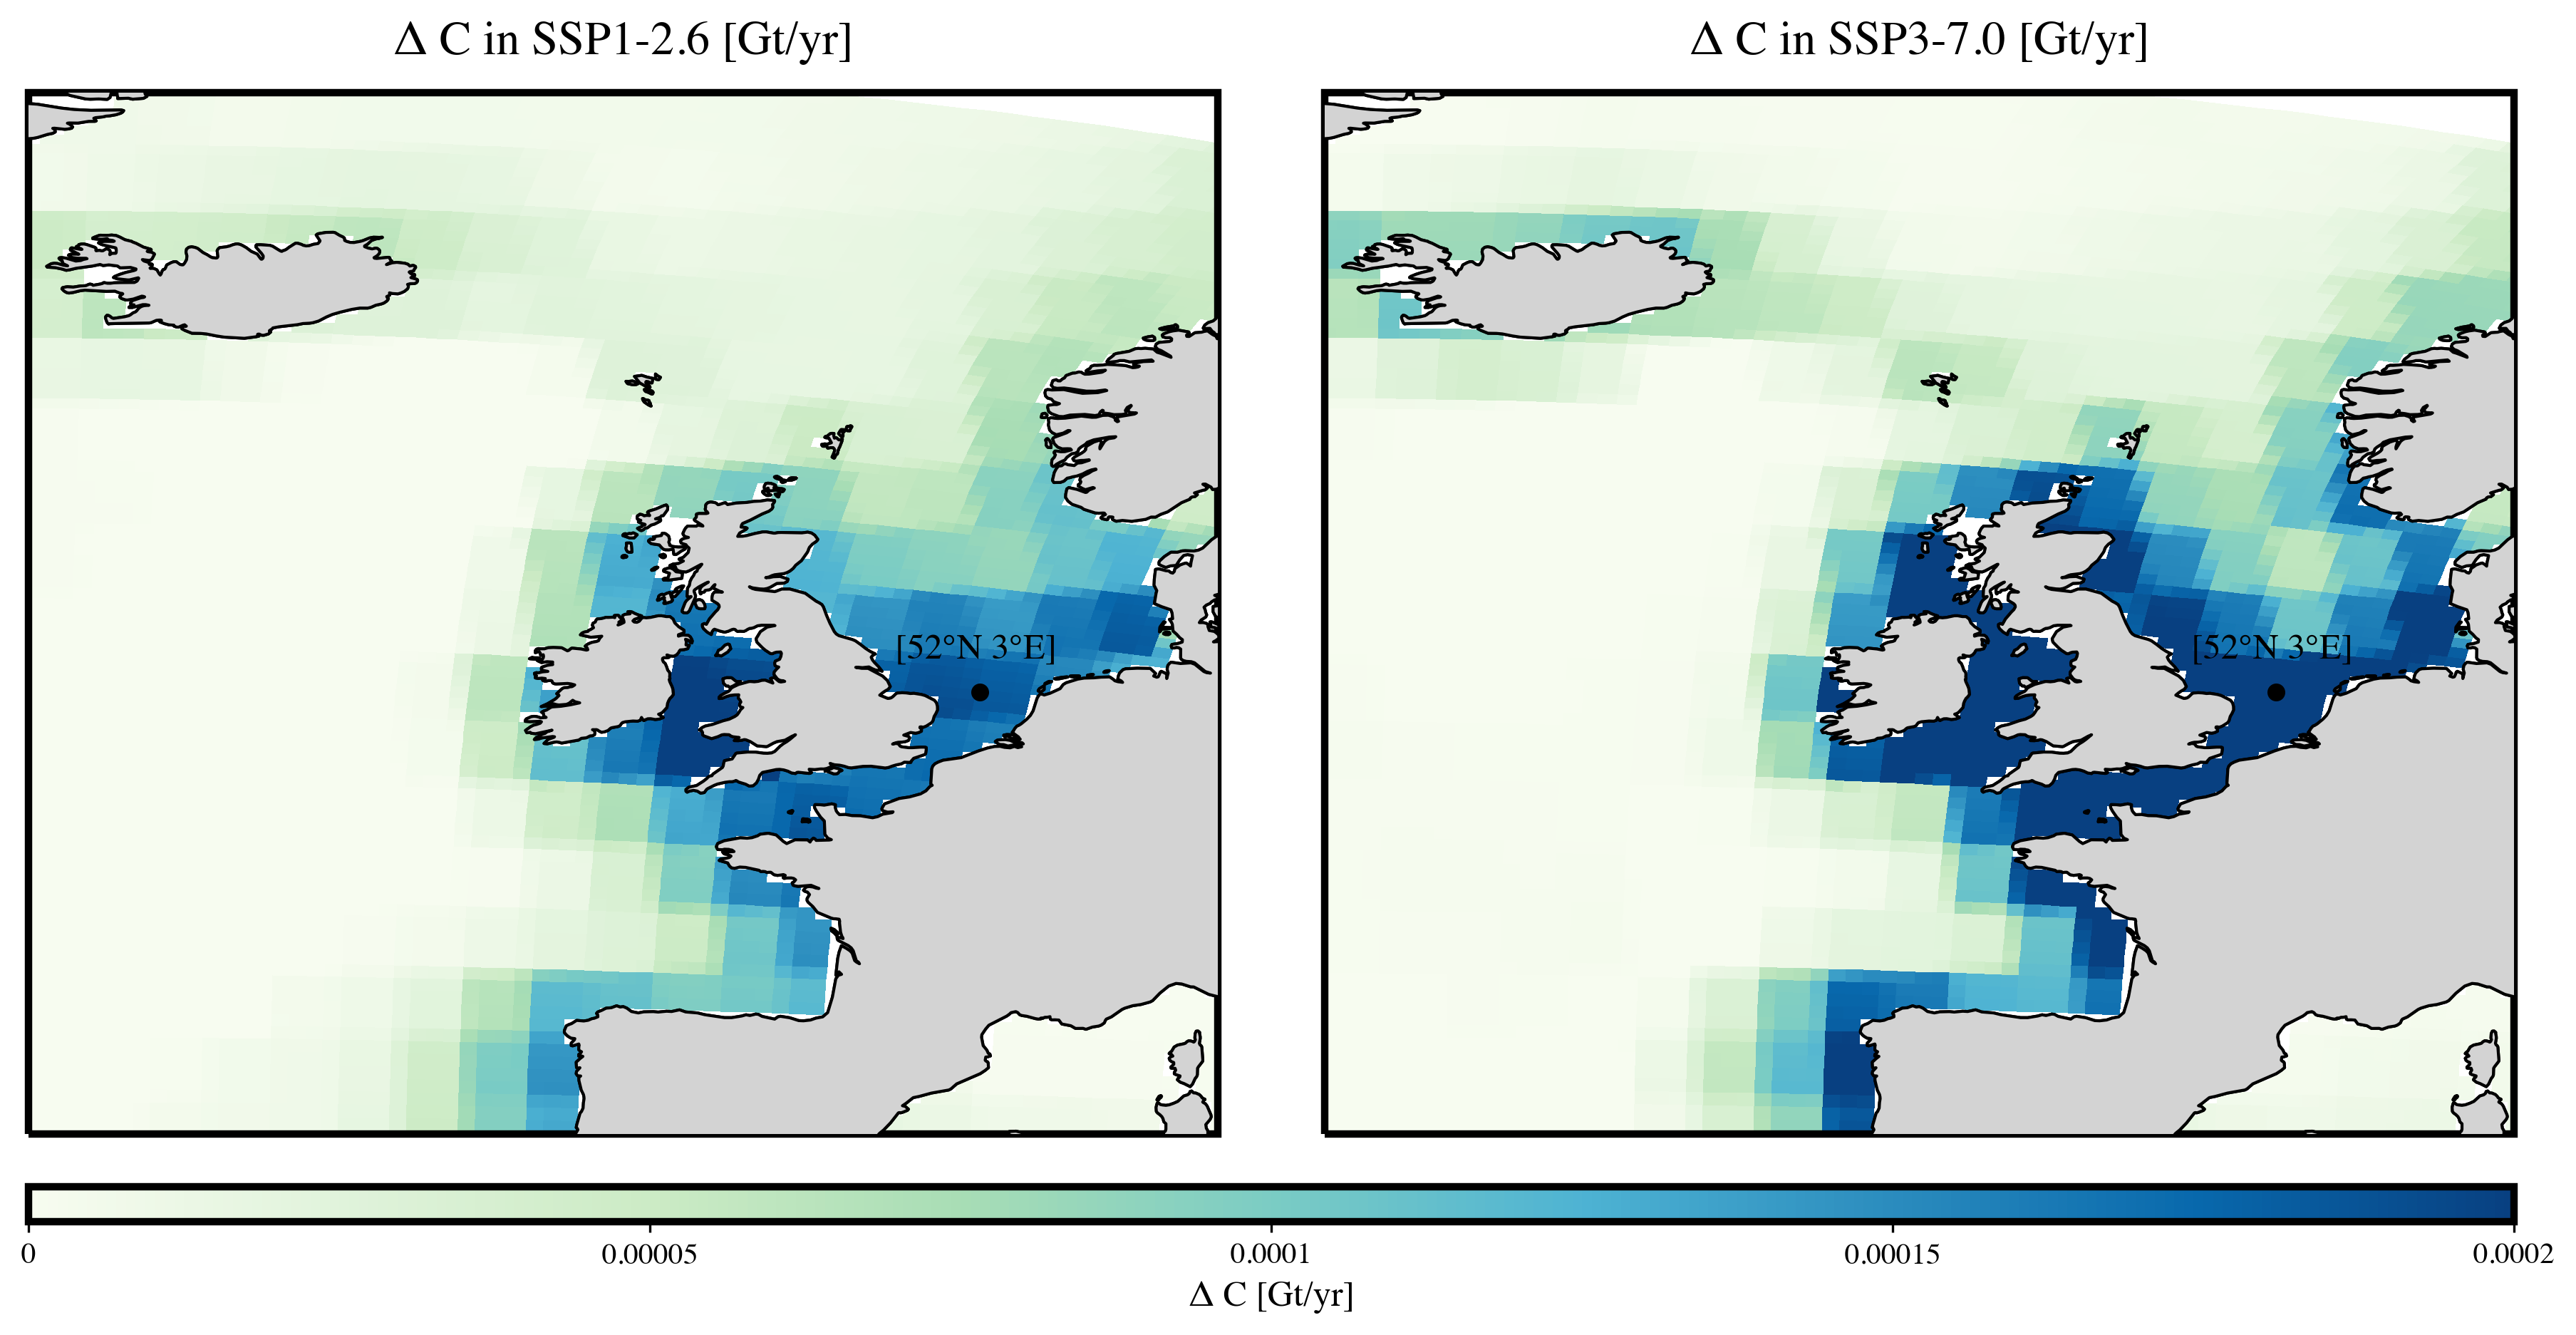
\includegraphics[width=15cm]{fig/3_Results/CO2flux/Cgt.png}

\end{figure}

In order to determine the magnitude of \ac{oae} impacts on the \ch{CO2} flux in European waters, the baseline-to-\ac{oae} change in carbon inventory in Gt yr\textsuperscript{-1} averaged over the last simulation decade was plotted (\cref{cgt}). It was found that \ac{oae} implementation has an additional uptake potential of 0.1779 GtC yr\textsuperscript{-1} in SSP1-2.6, which increases to 0.24 GtC yr\textsuperscript{-1} in SSP3-7.0. Following the definition in \cite{NAP26278}, where medium-to-high potential is set to a minimum threshold of 0.1–1.0 Gt \ch{CO2} yr\textsuperscript{-1}, these results confirm that \ac{oae} is expected to become an efficient tool for climate mitigation and reach net negative emissions. Additionally, the maps show that the southern North Sea offers an ideal location for \ac{oae} testing and similar regions should be viewed as the primary targets. 

